%%
%% This is file `sample-sigconf.tex',
%% generated with the docstrip utility.
%%
%% The original source files were:
%%
%% samples.dtx  (with options: `all,proceedings,bibtex,sigconf')
%% 
%% IMPORTANT NOTICE:
%% 
%% For the copyright see the source file.
%% 
%% Any modified versions of this file must be renamed
%% with new filenames distinct from sample-sigconf.tex.
%% 
%% For distribution of the original source see the terms
%% for copying and modification in the file samples.dtx.
%% 
%% This generated file may be distributed as long as the
%% original source files, as listed above, are part of the
%% same distribution. (The sources need not necessarily be
%% in the same archive or directory.)
%%
%%
%% Commands for TeXCount
%TC:macro \cite [option:text,text]
%TC:macro \citep [option:text,text]
%TC:macro \citet [option:text,text]
%TC:envir table 0 1
%TC:envir table* 0 1
%TC:envir tabular [ignore] word
%TC:envir displaymath 0 word
%TC:envir math 0 word
%TC:envir comment 0 0
%%
%%
%% The first command in your LaTeX source must be the \documentclass
%% command.
%%
%% For submission and review of your manuscript please change the
%% command to \documentclass[manuscript, screen, review]{acmart}.
%%
%% When submitting camera ready or to TAPS, please change the command
%% to \documentclass[sigconf]{acmart} or whichever template is required
%% for your publication.
%%
%%
\documentclass[sigconf, screen]{acmart}

%%
%% \BibTeX command to typeset BibTeX logo in the docs
\AtBeginDocument{%
  \providecommand\BibTeX{{%
    Bib\TeX}}}

%% Rights management information.  This information is sent to you
%% when you complete the rights form.  These commands have SAMPLE
%% values in them; it is your responsibility as an author to replace
%% the commands and values with those provided to you when you
%% complete the rights form.
\setcopyright{none} 
%\setcopyright{acmlicensed}
\copyrightyear{2024}
\acmYear{2024}
\acmDOI{XXXXXXX.XXXXXXX}

%% These commands are for a PROCEEDINGS abstract or paper.
\acmConference[`ISCA 2025']{The 52nd IEEE/ACM International Symposium on Computer Architecture}{June 21--25, 2025}{Tokyo, Japan}
%%
%%  Uncomment \acmBooktitle if the title of the proceedings is different
%%  from ``Proceedings of ...''!
%%
%%\acmBooktitle{Woodstock '18: ACM Symposium on Neural Gaze Detection,
%%  June 03--05, 2018, Woodstock, NY}
\acmISBN{978-1-4503-XXXX-X/18/06}


%%
%% Submission ID.
%% Use this when submitting an article to a sponsored event. You'll
%% receive a unique submission ID from the organizers
%% of the event, and this ID should be used as the parameter to this command.
%%\acmSubmissionID{123-A56-BU3}

%%
%% For managing citations, it is recommended to use bibliography
%% files in BibTeX format.
%%
%% You can then either use BibTeX with the ACM-Reference-Format style,
%% or BibLaTeX with the acmnumeric or acmauthoryear sytles, that include
%% support for advanced citation of software artefact from the
%% biblatex-software package, also separately available on CTAN.
%%
%% Look at the sample-*-biblatex.tex files for templates showcasing
%% the biblatex styles.
%%

%%
%% The majority of ACM publications use numbered citations and
%% references.  The command \citestyle{authoryear} switches to the
%% "author year" style.
%%
%% If you are preparing content for an event
%% sponsored by ACM SIGGRAPH, you must use the "author year" style of
%% citations and references.
%% Uncommenting
%% the next command will enable that style.
%%\citestyle{acmauthoryear}
\settopmatter{printfolios=true}
\settopmatter{printacmref=false}
%\pagestyle{plain}

\usepackage{makecell}
\usepackage{multirow} 
\usepackage[normalem]{ulem}
\usepackage[linesnumbered, ruled, vlined]{algorithm2e}
\usepackage{pifont}
\usepackage{amsfonts}
\usepackage{framed}
\usepackage{graphicx}
\newcommand{\bone}{\ding{182}}
\newcommand{\btwo}{\ding{183}}
\newcommand{\bthree}{\ding{184}}
\newcommand{\bfour}{\ding{185}}
\newcommand{\bfive}{\ding{186}}
\newcommand{\bsix}{\ding{187}}
\newcommand{\bseven}{\ding{188}}
\newcommand{\beight}{\ding{189}}
\newcommand{\bnine}{\ding{190}}
\newcommand{\bten}{\ding{191}}
\newcommand{\beleven}{\ding{192}}

\newcommand{\blfootnote}[1]{%
  \begingroup
  \renewcommand\thefootnote{}\footnote{#1}%
  \addtocounter{footnote}{-1}%
  \endgroup
}

\renewcommand\footnotetextcopyrightpermission[1]{}

%%
%% end of the preamble, start of the body of the document source.
\begin{document}

%%
%% The "title" command has an optional parameter,
%% allowing the author to define a "short title" to be used in page headers.
\title{FPGA-based Emulation and Device-Side Management for CXL-based Memory Tiering Systems}

% 添加作者和单位
\author{
{Yiqi Chen\textsuperscript{*1}, Xiping Dong\textsuperscript{*1}, Zhe Zhou\textsuperscript{1,2}, Zhao Wang\textsuperscript{1,2}, Jie Zhang\textsuperscript{2},  Guangyu Sun\textsuperscript{$\dagger$}\textsuperscript{1}} \vspace{0.5em} \\
% Dimin Niu\textsuperscript{2}, Hongzhong Zheng\textsuperscript{2}\\\\
\textsuperscript{1}\emph{School of Integrated Circuits}, \textsuperscript{2}\emph{School of Computer Science}, 
\emph{Peking University}\\
\emph{\{yiqi.chen, zhou.zhe, wangzhao21, jiez, gsun\}@pku.edu.cn} \\  \emph{dxp@stu.pku.edu.cn}\\
}

% \subtitle{\normalsize{ISCA 2025 Submission
%     \textbf{\#1125} -- Confidential Draft -- Do NOT Distribute!!}}
%%
%% The "author" command and its associated commands are used to define
%% the authors and their affiliations.
%% Of note is the shared affiliation of the first two authors, and the
%% "authornote" and "authornotemark" commands
%% used to denote shared contribution to the research.
%\author{\normalsize{ISCA 2025 Submission
 %   \textbf{\#NaN} -- Confidential Draft -- Do NOT Distribute!!}}

%%
%% By default, the full list of authors will be used in the page
%% headers. Often, this list is too long, and will overlap
%% other information printed in the page headers. This command allows
%% the author to define a more concise list
%% of authors' names for this purpose.

%%
%% The abstract is a short summary of the work to be presented in the
%% article.

\fancyhf{}


\begin{abstract}
\label{sec:abstract}
\begin{abstract}  
Test time scaling is currently one of the most active research areas that shows promise after training time scaling has reached its limits.
Deep-thinking (DT) models are a class of recurrent models that can perform easy-to-hard generalization by assigning more compute to harder test samples.
However, due to their inability to determine the complexity of a test sample, DT models have to use a large amount of computation for both easy and hard test samples.
Excessive test time computation is wasteful and can cause the ``overthinking'' problem where more test time computation leads to worse results.
In this paper, we introduce a test time training method for determining the optimal amount of computation needed for each sample during test time.
We also propose Conv-LiGRU, a novel recurrent architecture for efficient and robust visual reasoning. 
Extensive experiments demonstrate that Conv-LiGRU is more stable than DT, effectively mitigates the ``overthinking'' phenomenon, and achieves superior accuracy.
\end{abstract}  
\end{abstract}

%%
%% The code below is generated by the tool at http://dl.acm.org/ccs.cfm.
%% Please copy and paste the code instead of the example below.
%%
%\begin{CCSXML}
%<ccs2012>
% <concept>
%  <concept_id>00000000.0000000.0000000</concept_id>
%  <concept_desc>Do Not Use This Code, Generate the Correct Terms for Your Paper</concept_desc>
%  <concept_significance>500</concept_significance>
% </concept>
% <concept>
%  %<concept_id>00000000.00000000.00000000</concept_id>
%  <concept_desc>Do Not Use This Code, Generate the Correct Terms for Your Paper</concept_desc>
%  <concept_significance>300</concept_significance>
% </concept>
% <concept>
%  %<concept_id>00000000.00000000.00000000</concept_id>
%  <concept_desc>Do Not Use This Code, Generate the Correct Terms for Your Paper</concept_desc>
%  <concept_significance>100</concept_significance>
% </concept>
% <concept>
 % <concept_id>00000000.00000000.00000000</concept_id>
%  <concept_desc>Do Not Use This Code, Generate the Correct Terms for Your Paper</concept_desc>
%  <concept_significance>100</concept_significance>
% </concept>
%</ccs2012>
%\end{CCSXML}

%\ccsdesc[500]{Do Not Use This Code~Generate the Correct Terms for Your Paper}
%\ccsdesc[300]{Do Not Use This Code~Generate the Correct Terms for Your Paper}
%\ccsdesc{Do Not Use This Code~Generate the Correct Terms for Your Paper}
%\ccsdesc[100]{Do Not Use This Code~Generate the Correct Terms for Your Paper}

%%
%% Keywords. The author(s) should pick words that accurately describe
%% the work being presented. Separate the keywords with commas.
% \keywords{CXL, Memory Tiering System, Emulation Platform, FPGA}


%\received{20 February 2007}
%\received[revised]{12 March 2009}
%\received[accepted]{5 June 2009}
%%
%% This command processes the author and affiliation and title
%% information and builds the first part of the formatted document.
\maketitle

\section{Introduction}
\label{sec:introduction}
\section{Introduction}
\label{sec:introduction}
The business processes of organizations are experiencing ever-increasing complexity due to the large amount of data, high number of users, and high-tech devices involved \cite{martin2021pmopportunitieschallenges, beerepoot2023biggestbpmproblems}. This complexity may cause business processes to deviate from normal control flow due to unforeseen and disruptive anomalies \cite{adams2023proceddsriftdetection}. These control-flow anomalies manifest as unknown, skipped, and wrongly-ordered activities in the traces of event logs monitored from the execution of business processes \cite{ko2023adsystematicreview}. For the sake of clarity, let us consider an illustrative example of such anomalies. Figure \ref{FP_ANOMALIES} shows a so-called event log footprint, which captures the control flow relations of four activities of a hypothetical event log. In particular, this footprint captures the control-flow relations between activities \texttt{a}, \texttt{b}, \texttt{c} and \texttt{d}. These are the causal ($\rightarrow$) relation, concurrent ($\parallel$) relation, and other ($\#$) relations such as exclusivity or non-local dependency \cite{aalst2022pmhandbook}. In addition, on the right are six traces, of which five exhibit skipped, wrongly-ordered and unknown control-flow anomalies. For example, $\langle$\texttt{a b d}$\rangle$ has a skipped activity, which is \texttt{c}. Because of this skipped activity, the control-flow relation \texttt{b}$\,\#\,$\texttt{d} is violated, since \texttt{d} directly follows \texttt{b} in the anomalous trace.
\begin{figure}[!t]
\centering
\includegraphics[width=0.9\columnwidth]{images/FP_ANOMALIES.png}
\caption{An example event log footprint with six traces, of which five exhibit control-flow anomalies.}
\label{FP_ANOMALIES}
\end{figure}

\subsection{Control-flow anomaly detection}
Control-flow anomaly detection techniques aim to characterize the normal control flow from event logs and verify whether these deviations occur in new event logs \cite{ko2023adsystematicreview}. To develop control-flow anomaly detection techniques, \revision{process mining} has seen widespread adoption owing to process discovery and \revision{conformance checking}. On the one hand, process discovery is a set of algorithms that encode control-flow relations as a set of model elements and constraints according to a given modeling formalism \cite{aalst2022pmhandbook}; hereafter, we refer to the Petri net, a widespread modeling formalism. On the other hand, \revision{conformance checking} is an explainable set of algorithms that allows linking any deviations with the reference Petri net and providing the fitness measure, namely a measure of how much the Petri net fits the new event log \cite{aalst2022pmhandbook}. Many control-flow anomaly detection techniques based on \revision{conformance checking} (hereafter, \revision{conformance checking}-based techniques) use the fitness measure to determine whether an event log is anomalous \cite{bezerra2009pmad, bezerra2013adlogspais, myers2018icsadpm, pecchia2020applicationfailuresanalysispm}. 

The scientific literature also includes many \revision{conformance checking}-independent techniques for control-flow anomaly detection that combine specific types of trace encodings with machine/deep learning \cite{ko2023adsystematicreview, tavares2023pmtraceencoding}. Whereas these techniques are very effective, their explainability is challenging due to both the type of trace encoding employed and the machine/deep learning model used \cite{rawal2022trustworthyaiadvances,li2023explainablead}. Hence, in the following, we focus on the shortcomings of \revision{conformance checking}-based techniques to investigate whether it is possible to support the development of competitive control-flow anomaly detection techniques while maintaining the explainable nature of \revision{conformance checking}.
\begin{figure}[!t]
\centering
\includegraphics[width=\columnwidth]{images/HIGH_LEVEL_VIEW.png}
\caption{A high-level view of the proposed framework for combining \revision{process mining}-based feature extraction with dimensionality reduction for control-flow anomaly detection.}
\label{HIGH_LEVEL_VIEW}
\end{figure}

\subsection{Shortcomings of \revision{conformance checking}-based techniques}
Unfortunately, the detection effectiveness of \revision{conformance checking}-based techniques is affected by noisy data and low-quality Petri nets, which may be due to human errors in the modeling process or representational bias of process discovery algorithms \cite{bezerra2013adlogspais, pecchia2020applicationfailuresanalysispm, aalst2016pm}. Specifically, on the one hand, noisy data may introduce infrequent and deceptive control-flow relations that may result in inconsistent fitness measures, whereas, on the other hand, checking event logs against a low-quality Petri net could lead to an unreliable distribution of fitness measures. Nonetheless, such Petri nets can still be used as references to obtain insightful information for \revision{process mining}-based feature extraction, supporting the development of competitive and explainable \revision{conformance checking}-based techniques for control-flow anomaly detection despite the problems above. For example, a few works outline that token-based \revision{conformance checking} can be used for \revision{process mining}-based feature extraction to build tabular data and develop effective \revision{conformance checking}-based techniques for control-flow anomaly detection \cite{singh2022lapmsh, debenedictis2023dtadiiot}. However, to the best of our knowledge, the scientific literature lacks a structured proposal for \revision{process mining}-based feature extraction using the state-of-the-art \revision{conformance checking} variant, namely alignment-based \revision{conformance checking}.

\subsection{Contributions}
We propose a novel \revision{process mining}-based feature extraction approach with alignment-based \revision{conformance checking}. This variant aligns the deviating control flow with a reference Petri net; the resulting alignment can be inspected to extract additional statistics such as the number of times a given activity caused mismatches \cite{aalst2022pmhandbook}. We integrate this approach into a flexible and explainable framework for developing techniques for control-flow anomaly detection. The framework combines \revision{process mining}-based feature extraction and dimensionality reduction to handle high-dimensional feature sets, achieve detection effectiveness, and support explainability. Notably, in addition to our proposed \revision{process mining}-based feature extraction approach, the framework allows employing other approaches, enabling a fair comparison of multiple \revision{conformance checking}-based and \revision{conformance checking}-independent techniques for control-flow anomaly detection. Figure \ref{HIGH_LEVEL_VIEW} shows a high-level view of the framework. Business processes are monitored, and event logs obtained from the database of information systems. Subsequently, \revision{process mining}-based feature extraction is applied to these event logs and tabular data input to dimensionality reduction to identify control-flow anomalies. We apply several \revision{conformance checking}-based and \revision{conformance checking}-independent framework techniques to publicly available datasets, simulated data of a case study from railways, and real-world data of a case study from healthcare. We show that the framework techniques implementing our approach outperform the baseline \revision{conformance checking}-based techniques while maintaining the explainable nature of \revision{conformance checking}.

In summary, the contributions of this paper are as follows.
\begin{itemize}
    \item{
        A novel \revision{process mining}-based feature extraction approach to support the development of competitive and explainable \revision{conformance checking}-based techniques for control-flow anomaly detection.
    }
    \item{
        A flexible and explainable framework for developing techniques for control-flow anomaly detection using \revision{process mining}-based feature extraction and dimensionality reduction.
    }
    \item{
        Application to synthetic and real-world datasets of several \revision{conformance checking}-based and \revision{conformance checking}-independent framework techniques, evaluating their detection effectiveness and explainability.
    }
\end{itemize}

The rest of the paper is organized as follows.
\begin{itemize}
    \item Section \ref{sec:related_work} reviews the existing techniques for control-flow anomaly detection, categorizing them into \revision{conformance checking}-based and \revision{conformance checking}-independent techniques.
    \item Section \ref{sec:abccfe} provides the preliminaries of \revision{process mining} to establish the notation used throughout the paper, and delves into the details of the proposed \revision{process mining}-based feature extraction approach with alignment-based \revision{conformance checking}.
    \item Section \ref{sec:framework} describes the framework for developing \revision{conformance checking}-based and \revision{conformance checking}-independent techniques for control-flow anomaly detection that combine \revision{process mining}-based feature extraction and dimensionality reduction.
    \item Section \ref{sec:evaluation} presents the experiments conducted with multiple framework and baseline techniques using data from publicly available datasets and case studies.
    \item Section \ref{sec:conclusions} draws the conclusions and presents future work.
\end{itemize}

\section{Background \& Motivation}
\label{sec:background}
\section{Related Works}
\label{sec:background_motivation}
%\vspace{-1mm}
%3GPP employs dynamic scheduling to allocate resources to UEs in the time domain, representing the prevalent method in commercial cellular networks\,\cite{fezeu2023depth}. Our proposed solution builds upon this approach, aiming to enhance its efficacy.
%\vspace{-1mm}
%\subsection{Related Works \textcolor{red}{(to-do)}}
\textcolor{red}{to-do}Existing studies investigate 5G performance improvements through layer specific optimization solutions, such as application layer solutions [cite], RLC layer solutions [cite], MAC layer solutions [cite], and PHY layer solutions [cite]. Studies such as [cite] investigate the effect of 5G on emerging human-centric applications such as XR and propose application-aware network layer solutions such as PDU sets, but these solutions are for a specific class of applications and are confined to a specific layer of the network stack. Overall, these studies do not consider emerging machine-centric application requirements and also do not explore the effect of joint optimization across the different layers of the network stack through a learnable approach.
%\subsection{Legacy 5G network optimization}
\vspace{-1mm}
%A frame in 5G is 10\,ms long, which is broken down into 10 subframes. Depending on the numerology, the number of slots in a subframe varies. Here, we consider a subframe of 30\,KHz subcarrier spacing (SCS) spanning two slots. In TDD, the DL-UL-periodicity determines the time for which there can be a consecutive set of DL and UL slots. Each slot is further broken down into 14 symbols assuming a normal cyclic prefix (CP). 
\begin{comment}
\noindent $\bullet$ \textbf{Time domain resource allocation: }For allocating resources in the time domain in 5G, the NW informs the UE about which slots/symbols can be used for data transmission/reception through signaling of time-domain resources using DCI in PDCCH. In 5G, DCI formats [{0\_0}] and [{0\_1}] allocate time-domain resources for UL data in the physical uplink shared channel (PUSCH). DCI formats {0\_0} and {0\_1} carry a 4-bit field named ‘time domain resource assignment’ which points to one of the 16 rows of a look-up table\,\cite{snr-cqi-mcs}. Each row in the look-up table provides the following parameters:
\begin{figure}[t!]
	\centering
	\includegraphics[trim=0 0 0 0,clip,width=\linewidth]{Figures/time_domain_allocation.pdf}
	\vspace{-2mm}
	\caption{Example time domain resource assignment from NW to UE in 5G.}
 \vspace{-4mm}
	\label{fig:time_domain_alloc}
\end{figure}
\begin{itemize}
    \item \textit{Slot offset K2.} This parameter is used to derive the slot in which PUSCH transmission occurs.
    \item Jointly coded \textit{Start and Length Indicator Values (SLIV)}, or individual values for the start symbol $S$ and the allocation length $L$.
    \item \textit{PUSCH mapping type} to be applied on the PUSCH transmission.
\end{itemize}
\end{comment}
%\noindent $\bullet$ \textbf{Dynamic scheduling procedure: }
%The time domain resource allocation for UL transmission in 5G are shown in Fig.\,\ref{fig:time_domain_alloc}. 
%In TDD, the NW divides the time domain into either dedicated DL or UL or mixed/flexible (F) slots. Here, the UE first sends a scheduling request (SR) as control information in either a UL or an F slot, informing the NW of pending data to transmit. The UE informs the NW of the most recent channel estimates and the available data volume through the buffer status report (BSR) as control information\,\cite{3gppmac}. The NW after receiving these control data, informs the UE of the assigned resources via DCI, which indicates the specific slot, starting OFDM symbol, and symbol length in the following PHY frame for uplink data transmission. The UE then prepares the transport block sizes (TBS) based on the MCS and the assigned OFDM symbols and transmits the application data in the scheduled UL slots. 3GPP allows flexible scheduling in which slots are dedicated for DL vs. UL transmissions\,\cite{3gpprlc}.
%Existing 5G optimization techniques primarily focus on individual network layers. Application data flows through the network stack until it reaches the RLC buffer where it can accumulate due to wireless channel degradation, network congestion, etc. The RLC layer has FIFO queues (RLC channels) per application class [cite]. Packets wait at the RLC buffer until the MAC scheduler allocates Resource Blocks (RBs), in the network signaled PHY frame slots, to the data in the RLC buffer. This allocation process considers various factors such as channel conditions, application class KPI bounds, buffer status, etc. While commercial networks employ proprietary non-public MAC scheduling algorithms tailored to their specific needs, 3GPP provides standardized algorithms like \textit{Round Robin}, \textit{Proportional Fair}, and \textit{bestCQI} as benchmarks for evaluating new scheduling methods. Commercial 5G networks such as AT\&T, T-Mobile, and Verizon all configure the 5G PHY frame of 10\,ms duration, with the same {\em fixed} configuration that has more downlink (DL) than uplink (UL) slots\,\cite{fezeu:techreport2023}, leading to imbalanced traffic distribution. The resource allocation in the PHY layer is \textit{reactive}, where the UE triggers the dynamic scheduling process by transmitting a Scheduling Request (SR) to the NW in a UL or F slot, indicating pending UL data, and providing channel estimates via the physical uplink control channel (PUCCH)\,\cite{3gppmac}. Subsequently, the NW informs the UEs of resource allocation using downlink control information (DCI) in the downlink control channel (PDCCH). Here, among other things, the NW specifies slot assignments for UEs in the uplink service channel (PUSCH) and downlink service channel (PDSCH) for UL transmission and DL reception, respectively. 

%\noindent $\bullet$ \textbf {PHY layer:} The 5G PHY layer performance is based on the resource allocation in the PHY frames which are divided into DL and UL slots. Commercial 5G networks such as AT\&T, T-Mobile, and Verizon all configure the 5G PHY frame of 10\,ms duration, with the same {\em fixed} configuration that has more DL than UL slots\,\cite{fezeu:techreport2023}, leading to imbalanced traffic distribution.
%In TDD, the NW configures the PHY frame of 10\,ms duration into dedicated DL, UL, and mixed/flexible (F) slots in the time domain (20 slots per frame in this example), as shown in Fig.\,\ref{fig:7_2_1}. 
%The resource allocation in the PHY layer is \textit{reactive}, where the UE triggers the dynamic scheduling process by transmitting a Scheduling Request (SR) to the NW in a UL or F slot, indicating pending UL data, and providing channel estimates via the physical uplink control channel (PUCCH)\,\cite{3gppmac}. Subsequently, the NW informs the UEs of resource allocation using downlink control information (DCI) in the downlink control channel (PDCCH). Here, among other things, the NW specifies slot assignments for UEs in the uplink service channel (PUSCH) and downlink service channel (PDSCH) for UL transmission and DL reception, respectively. 

%\noindent $\bullet$ \textbf {MAC layer:} 
%The MAC scheduler at each base station (gNB) decides the UE-wise PRB allocation for every slot. In FDD, PDSCH and PUSCH allocations are output per slot, while in TDD, the appropriate (PDSCH or PUSCH) allocation is output every slot (DL or UL). The scheduler uses the information related to the SINR, CQI, MCS, number of MIMO layers, buffer status, and HARQ  as inputs for each gNB and attached UE. The scheduler also uses the number of PRBs available in the gNB. Re-transmissions are prioritized over first transmissions. The scheduler's output is UE-wise PRB allocation in the UL and DL, at every slot. MAC scheduling algorithms in commercial networks are customized for specific business needs and are unavailable in the public domain. 3GPP provides some baseline MAC scheduling algorithms (Round Robin, Proportional Fair, and bestCQI) for evaluating the performance of proposed methods in the upstream and downstream functions. The \textit{RoundRobin} method divides the available PRBs among the logical channels that have a non-empty RLC queue. The MCS for each user is calculated according to the received CQIs. The \textit{Proportional Fair} method works by scheduling a (active) user when its instantaneous channel quality is high relative to its own average channel condition over time. The PF scheme is based on the current data rate for each user and the exponentially weighted moving average (EWMA) data rate over an immediately prior predetermined interval for each user. In comparison with the round-robin (RR) scheduler in which UEs are cyclically scheduled irrespective of the channel condition, the PF scheduler maximizes the system throughput while maintaining long-term fairness in the allocation of resources between users. The \textit{bestCQI} method allocates PRBs to the active flow(s) to maximize the achievable rate. It selects the user that sees the highest CQI.
%In the 5G MAC layer, the scheduler at each base station (gNB) allocates Physical Resource Blocks (PRBs) to User Equipments (UEs) for every time slot. This allocation process considers various factors such as Signal-to-Interference-plus-Noise Ratio (SINR), Channel Quality Indicator (CQI), Modulation and Coding Scheme (MCS), number of Multiple-Input Multiple-Output (MIMO) layers, buffer status, and Hybrid Automatic Repeat reQuest (HARQ) information. 
%The scheduler prioritizes re-transmissions over first transmissions to ensure data reliability. 
%While commercial networks employ proprietary non-public MAC scheduling algorithms tailored to their specific needs, 3GPP provides standardized algorithms like \textit{Round Robin}, \textit{Proportional Fair}, and \textit{bestCQI} as benchmarks for evaluating new scheduling methods. 
%The Round Robin algorithm distributes PRBs equally among active logical channels, while the Proportional Fair algorithm dynamically allocates resources to users with favorable instantaneous channel conditions relative to their average channel quality, thereby maximizing system throughput and ensuring long-term fairness. The \textit{bestCQI} algorithm prioritizes the user with the highest CQI to maximize the achievable data rate.

%\noindent $\bullet$ \textbf {Application layer:} 
%Flexible  scheduling, sanctioned by 3GPP, assigns slots for DL and UL transmissions as needed.

%Commercial 5G networks such as AT\&T, T-Mobile, and Verizon all use the same {\em fixed} PHY frame configuration that has more DL than UL slots -- 7\,DL-2\,UL-1\,F (7\,DL 3\,UL)\,\cite{fezeu:techreport2023}, with a periodicity of 5\,ms (Fig.\,\ref{fig:7_2_1}), leading to imbalanced traffic distribution.
%Existing drive-test studies on these commercial networks using 5G smartphones reveal impressive DL speeds, surpassing 3.5\,Gbps, while UL throughput remains consistently lower\,\cite{ghoshal:imc2023}. The fixed DL-heavy PHY frame configuration may strain 5G networks, particularly with the rise of uplink-heavy applications. The use of this fixed PHY frame configuration persists due to the prevalence of existing DL-heavy applications and the 3GPP-supported {\em reactive} scheduling method based on UE-reported channel metrics. The lack of channel forecast knowledge provides little incentive for the NW to modify PHY frame configuration relying solely on UE-reported channel metrics as this process may take time to converge and can result in sub-optimal NW performance. 
\vspace{-1mm}


\section{HeteroBox Platform}
\label{sec:heterobox}
\begin{figure*} [t]
    \centering
    \includegraphics[width=1.0\linewidth]{fig/heterobox.pdf} 
    % \vspace{-1.2em}
    \vspace{-0.7cm}
    \caption{Overview of HeteroBox Emulation Platform.}
     \label{fig:heterobox_overview}
     \vspace{-0.4cm}
\end{figure*}

% \section{System Overview}
% \begin{teaserfigure}
    \centering
    \includegraphics[width=1\linewidth]{figures/hero_fig.png}
    \caption{Our system translates English text into a photorealistic ASL video with non-manual information. It starts with an English text input (first row), generates ASL tokens capturing both manual and non-manual details (second row), produces a skeletal pose sequence (third row), and finally creates the photorealistic ASL video (fourth row). \han{@all, please check the stylization.}}
    % \han{should we have a longer sentence? Ideally has 6-7 video frames. Still working on stylization...} \rotem{thinking about it again, instead of putting it here, I would have 1-2 examples here- only text->gloss->ours with expressions (or through pose), then have a no expression vs expression fig later on in the paper..}}
    \label{fig:system_overview}
\end{teaserfigure}

\section{HeteroMem Solution}
\label{sec:heteromem}
% In this section, we detail the hardware architecture of each component of the HeteroBox emulation platform and the HeteroMem memory tiering system.


\subsection{Overview of HeteroMem System}
\begin{figure}[t]
  \centering
  \includegraphics[width=\columnwidth]{fig/heterobox_system_overview.pdf}
  \vspace{-0.5cm}
  \caption{System Overview of HeteroMem}
  \vspace{-0.7cm}
  \label{fig:heterobox_system_overview}
\end{figure}

% The HeteroMem memory tiering system act as an intermediate layer between host CPU and device-side memory controller. The system is consisted of three main components: \textbf{Remap Table}, \textbf{Profile Unit} and \textbf{Migrate Unit}. Besides, we implement software interface support for the enumeration platform, including software driver in the kernel and BAR regs in the device for configuration and debugging. Without losing generality, in the following evaluation of HeteroMem memory tiering system, we use two tiers memory system, which consists of a fast memory tier and a slow memory tier.

% The HeteroMem memory tiering system acts as an intermediate layer between the host CPU and the device-side memory controller. 
The HeteroMem memory tiering system acts as an intermediate layer between host CPU and CXL-extended memory. 
As shown in Figure~\ref{fig:heterobox_system_overview}, the HeteroMem system comprises three main components: the \textbf{Remapping Unit}, the \textbf{Profiling Unit}, and the \textbf{Migration Unit}. 
% Additionally, we provide software interface support for the emulation platform, including a software driver in the kernel and BAR registers in the device for configuration and debugging. 
Additionally, we provide software interface support for HeteroMem memory tiering system, including a software driver in the kernel and BAR registers in the device for configuration and profiling. 
For the following evaluation of HeteroMem memory tiering system, we use a two-tier memory system, consisting of a fast memory tier and a slow memory tier, without losing generality.


% \begin{figure*} [t!]
%     \centering
    % \includegraphics[width=1.0\linewidth]{fig/remap_table_working_process.pdf} 
%     \vspace{-1.2em}
%     \caption{Remap Table Working Process.}
%          \label{fig:remap_table_working_process}
%          \vspace{-1em}
% \end{figure*}

\begin{figure*}[t!]
    \centering
    % \vspace*{-1.5cm}
    \includegraphics[width=1.0\linewidth]{fig/remap_table_working_process.pdf}
    \vspace{-0.7cm}
    \caption{Remapping Unit Working Process.}
    \label{fig:remap_table_working_process}
    \vspace*{-0.5cm}
\end{figure*}
\begin{figure}[t]
  \centering
  \includegraphics[width=\columnwidth]{fig/remap_table_v2.pdf}
  \vspace{-0.5cm}
  \caption{Block Diagram of the Remapping Unit}
  \vspace{-0.6cm}
  \label{fig:remap_table}
\end{figure}


\noindent{\textbf{Remapping Unit:}} 
% HeteroMem proposes to manage the heterogeneous memory system totally at device-side. This includes migrating the hot data from slow memory media to fast memory media, and migrating the cold data from fast memory media to slow memory media. As a result, the device needs to record the actual address of data when receiving a memory request issued by host. We build a remap table module to do this, which receives memory requests from host and translate the memory request to its actual address in the device, and then forward the translated request to the succeeding modules. The remap table should be carefully designed, because: 1) It is on the critical path of a memory request, which shouldn't introduce too much latency, otherwise it will affect the overall performance the memory system. 2) The translation granularity of remap table further determines the migration granularity, in which smaller granularity means larger overhead of remap table yet less migration amplification, larger granularity introduce less overhead in remap table yet cause more serious migration amplification. We will discuss these trade-offs of remap table in section~\ref{sec:heterobox_hardware}.
% HeteroMem proposes to manage the heterogeneous memory system entirely on the device side. This includes migrating hot data from slow memory media to fast memory media and migrating cold data from fast memory media to slow memory media. Consequently, the device must record the actual address of data when receiving a memory request from the host. We implement a Remap Unit module to handle this, which receives memory requests from the host, translates the memory request to its actual address in the device, and then forwards the translated request to the subsequent modules. The Remap Unit must be carefully designed since it is on the critical path of a memory request, and should not introduce significant latency, as this would affect the overall performance of the memory system. 
% 2) The translation granularity of the remap table determines the migration granularity. Smaller granularity results in larger overhead for the remap unit but less migration amplification, whereas larger granularity introduces less overhead in the remap table but causes more significant migration amplification. 
% We will discuss the design of Remap Unit in section~\ref{sec:heteromem}.
% \xp{also discuss remapping overhead in section~\ref{sec:evaluation}}
% HeteroMem manages the heterogeneous memory system entirely on the device side, including migrating hot data to fast memory and cold data to slow memory. 
% To keep the device side data migration transparent to CPU, the device needs a translation layer which can map the request address from host to its actual address in the device. 
% We implement a Remap Unit to handle this, translating memory requests to their actual addresses on the device and forwarding them to subsequent modules. Since the Remap Unit is on the critical path of a memory request, it must be carefully designed to avoid introducing significant latency, which would impact overall system performance.
HeteroMem manages heterogeneous memory system entirely on the device side, migrating hot data to fast memory and cold data to slow memory. To keep this migration transparent to CPU, the device needs a translation layer to map hPA to dPA. We implement a Remapping Unit to handle this, translating memory requests and forwarding them to subsequent modules. Since the Remapping Unit is on the critical path of memory requests, it must minimize added latency to ensure optimal system performance.


\noindent{\textbf{Profiling Unit:}} 
% To optimize the performance the heterogeneous memory system, we need to migrate the hot data to fast memory media. We build Profile Unit to measure the hotness of data at different address in the device. The Profile Unit take memory requests which are already translated by remap table as input and record this access. When the Profile Unit recognize data at a address as hot, it will issue a signal to remap table to indicate that a migration event should be executed. The signal contains a pair of address, which locate in fast memory region and slow memory region respectively. The Profile Unit should classify hot page and cold page accurately to do the right migration decision. For hot pages, we implement a sketch to evaluate the access time of each page and choose those with a access time larger than a threshold to be hot.
% Cold pages, however, are harder to detect. Building a LRU-like structure in a GB-level address space is impracticable because of it will consume large amount of hardware resource. Fortunately, cold page tends to remain cold in relatively longer time~\cite{tmts_asplos2023}. Based on this insight, we use a periodically scanning method to balance the hardware overhead and profiling accuracy.
% %For cold pages, we scan the address space periodically and choose those with smallest access time as cold pages.
% Besides, we design a dynamic hotness threshold setting mechanism to ensure that the hottest part of data remain in fast memory. We will discuss the design of Profile Unit in detail in section~\ref{sec:heterobox_hardware}.
% To optimize the performance of the heterogeneous memory system, we need to migrate hot data to fast memory media. We develop the Profile Unit to measure the hotness of data at different addresses in the CXL extended memory space. 
% The Profile Unit takes memory requests that have already been translated by the Remap Unit as input and records this access. When the Profile Unit identifies data at an address as hot, it issues a signal to the Remap Unit to indicate that a migration event should be executed. This signal contains a pair of addresses, located in the fast memory region and slow memory region, respectively. The Profile Unit must accurately classify hot pages and cold pages to make correct migration decisions. For hot pages, we implement a sketch to evaluate the access times of each page and select those with access times larger than a threshold to be considered hot.
% Detecting cold pages, however, is more challenging. Constructing an LRU-like structure in a GB-level address space is impractical due to the large amount of hardware resources it would consume. Fortunately, cold pages tend to remain cold for relatively longer periods~\cite{tmts_asplos2023}. Based on this insight, we use a periodic scanning method to balance hardware overhead and profiling accuracy. Additionally, we design a dynamic hotness threshold setting mechanism to ensure that the hottest portion of data remains in fast memory. 
% We will discuss the design of the Profile Unit in detail in section~\ref{sec:heteromem}.
% The Profile Unit is used for hotness and coldness profiling of the CXL-extended memory. The Profile Unit uses translated memory requests from the Remap Unit as input and records access patterns. The Profile Unit proactively profiles the data hotness in slow memory and data coldness in fast memory. Detected cold data will be temporarily buffered. When it identifies hot data, it signals the Remap Unit to initiate a migration event, providing a pair of hot data address and cold data address for the succeeding migration transaction.
% The Profile Unit profiles the hotness and coldness of data in CXL-extended memory using translated memory requests from the Remap Unit. It records access patterns and proactively profiles data hotness in slow memory and data coldness in fast memory, temporarily buffering detected cold data. When hot data is identified, the Profile Unit signals the Remap Unit to initiate a migration event, providing addresses for the hot data and previously buffered cold data for the migration transaction.
The Profiling Unit assesses the hotness and coldness of data in CXL-extended memory using translated memory requests from the Remapping Unit. It records access patterns, profiling hot data in slow memory and cold data in fast memory, temporarily buffering the dPA of detected cold data. When hot data is identified, the Profiling Unit signals Remapping Unit to initiate a migration event, providing the dPA for hot data and the dPA of previously buffered cold data for subsequent migration transaction.


\noindent{\textbf{Migration Unit:}} 
% The Migrate Unit is responsible for data migration. It takes in two address, corresponding to two pages, and it swap the content of these two pages. The key point in designing a Migrate Unit is that we need to keep all migration event transparent to CPU. To achieve that, we need to update the Remap Table when migration happens. Also, we need to ensure that at the when the Migrate Unit has already finished migrating data and the Remap Table has not updated its translation rule, no memory request can go through the Remap Table, being translated and sent to the DRAM module, otherwise it will cause broken data. We will discuss our design of Migrate Unit and how it co-operate with Remap Table in detail in section~\ref{sec:heterobox_hardware}.
% The Migrate Unit is responsible for data migration. 
% It takes in migration requests issued from Remap Unit, which contain two memory addresses corresponding to hot and cold data detected by Profile Unit, and swaps their memory location. 
% The key point in designing the Migrate Unit is to ensure that all migration events remain transparent to the CPU. To achieve this, we need to update the Remap Unit when migration occurs. Additionally, we must ensure that during the period when the Migrate Unit has finished migrating data but the Remap Unit has not yet updated its translation rules, no memory requests can pass through the Remap Unit, be translated, and be sent to the DRAM module; otherwise, this would result in data corruption. 
% We will discuss our design of the Migrate Unit and how it cooperates with the Remap Unit in detail in section~\ref{sec:heteromem}.
The Migration Unit initiates data migration upon receiving requests from the Remapping Unit, which contain dPAs for hot and cold data identified by the Profiling Unit, and swaps their memory locations. To keep migrations transparent to the CPU, the Remapping Unit must be updated whenever a migration occurs. 
% During this transaction, it is crucial to prevent memory requests from being translated by the Remapping Unit until the translation rules are updated to avoid data corruption.


% \noindent{\textbf{Latency Module:}} We build our enumeration platform on a FPGA board with homogeneous DRAM memory, yet we need to enumerate heterogeneous memory system with different configuration, such as different capacity ratio and different latency. To achieve that, we build a Latency module as an abstract layer between memory controller and other logic. It can be configured to devide the DRAM into two regions, which make an illusion that the two regions has different latency attribute, thus forming a abstraction of heterogeneous memory system with two-tiered memory. We will discuss the design of Latency Module in detail in section ?. 





\subsection{Remapping Unit}


% The Remap Table provides an additional translation layer between CPU and device. It needs to carefully designed to introduce low overhead and keep the translation process transparent to CPU. 
The Remapping Unit provides an additional translation layer between the CPU and the device. It needs to be carefully designed to introduce minimal overhead and keep the translation process transparent to the CPU.

\noindent{\textbf{Memory Layout:}} 
% As shown in Figure \ref{fig:remap_table_working_process}, the whole memory space is consisted of 1GB of fast memory and 15GB of slow memory. We modify the Linux kernel to software reserve the first 128MB of the fast memory. When the machine power on, the remap table will send a series of write request to the reserved fast memory to initialize the remap table meta data. The remap table meta data consists of a remap table array and a reversed remap table array. Access the remap table array with the index of a page index will get the translated page index corresponding to the original page index. The reversed remap table is responsible for the reversed translation.
% As shown in Figure \ref{fig:remap_table_working_process}-(a), the entire memory space consists of a fast memory region and a slow memory region. 
% The Remap Unit stores the metadata used for address translation at the beginning of fast memory.
% The memory used to store metadata is software reserved to avoid being accessed by host CPU.
% When the machine powers on, the Remap Unit sends a series of write requests to the reserved fast memory to initialize the metadata.
% This metadata consists of a remap table array and a reverse remap table array. 
% Both remap table array and reverse remap table array consist of 4 bytes entries, each entry contains a page index. Using 4 bytes page index can describe a memory space up to 16TB, and we can use longer page index (for example, 8 bytes) for larger memory space.
% Accessing the remap table array with a page index yields the translated page index corresponding to the original page index, while the reverse remap table contains the inverse mapping of the remap table. 
As shown in Figure \ref{fig:remap_table_working_process}-(a), the entire memory space consists of a fast memory region and a slow memory region. 
The Remapping Unit stores the metadata for address translation at the beginning of the fast memory, which is software-reserved to avoid access by the host CPU. 
When the machine powers on, the Remapping Unit initializes this metadata by sending a series of write requests to the reserved fast memory.
This metadata includes a remapping table array and a reverse remapping table array, both consisting of 4-byte entries, each containing a page index (for dPA). 
% HeteroMem manages the memory in 4KB granularity, so a 4-byte page index can describe a memory space of up to 16TB, and a longer index (e.g., 8 bytes) can be used for larger memory space. 
HeteroMem manages memory in 4KB page granularity, so a 4-byte page index can describe a memory space of up to 16TB. For larger memory spaces, a longer index (e.g., 8 bytes) can be used.
Accessing the remapping table array with a page index yields the translated page index, while the reverse remapping table contains the inverse mapping of the remapping table.


\noindent{\textbf{Architecture of Remapping Unit:}} 
% The architecture of the Remap Table is shown in Figure \ref{fig:remap_table}. When a memory request is issued to the Remap Table, it first come into a remap cache which buffers the remap table meta data stored in the memory. If the cache contains the meta data which is needed to translate the current request, the remap table translate the current request with the meta data and send it to the memory. If the cache miss, the current request will be buffered in a fifo to pipelining the translation process of the succeeding requests, and the remap cache will issue a read request to the remap table data in the memory. When the response of the read request returned to the remap table, the remap cache will be updated, and the request buffered in the fifo will be translated and sent to the memory. 
% The architecture of the Remap Unit is shown in Figure \ref{fig:remap_table}. When a memory request is issued to the Remap Unit, it first enters a remap cache, which buffers the remap table metadata stored in the memory. If the cache contains the metadata needed to translate the current request, the Remap Unit translates the request using the metadata and sends it to the memory. If there is a cache miss, the current request is buffered in a FIFO to pipeline the translation process for subsequent requests, and the remap cache issues a read request to fetch the remap table data from the memory. Once the read request response returns to the Remap Unit, the remap cache is updated, and the request buffered in the FIFO is translated and sent to the memory.
% The architecture of the Remapping Unit is shown in Figure \ref{fig:remap_table}. When a memory request reaches the Remapping Unit, it first enters a remapping cache that buffers the remapping table metadata stored in memory. If the cache contains the necessary metadata to translate the request, the Remapping Unit performs the translation and forwards the request to memory. In the case of a remapping cache miss, the current request is buffered in a FIFO to pipeline the translation process for subsequent requests, and the remapping cache issues a read request to fetch the remapping table data from memory. Once the read response returns, the remapping cache is updated, and the buffered request in the FIFO is translated and sent to memory.
% Figure~\ref{fig:remap_table_working_process}-(b) shows the translation process of Remap Unit when a remap cache miss happens.
The Remapping Unit's architecture, shown in Figure \ref{fig:remap_table}, works as follows: when a memory request arrives, it first checks the remapping cache, which stores metadata for translating requests. If the required metadata is found, the request is translated and sent to memory. On a cache miss, the request is buffered in a FIFO, and the remapping cache issues a memory read to retrieve the needed remapping table data. Once the data returns, the cache is updated, and the buffered request is translated and forwarded to memory.
Figure~\ref{fig:remap_table_working_process}-(b) illustrates the translation process of the Remapping Unit when a remapping cache miss occurs.



\begin{figure*} [t]
    \centering
    \includegraphics[width=0.9\linewidth]{fig/profile_unit.pdf} 
    % \vspace{-1.2em}
    \vspace{-0.4cm}
    \caption{Profiling Unit Overview.}
     \label{fig:profiling_unit_overview}
     \vspace{-0.4cm}
\end{figure*}

\noindent{\textbf{Migration Transaction:}} 
% As shown in Figure \ref{fig:remap_table_working_process}.b, when the remap table receive a migration request from the profile unit(\bone), it will start a migration transaction. The migration request contains a pair of page index which locate in fast memory and slow memory respectively. The page index in the migration request is page index which is already translated. Upon receive the migration request, the remap table will block the succeeding request from the host to ensure the atomic attribute of the migration. Then, remap table will issue a memory read request to the reverse remap table in the memory to get the original request address(\btwo). When the read response containing the original request address returns(\bthree), the remap table will update the remap table data and reverse remap table data according to the two original address and two translated address(\bfour). The Remap Table will concurrently send an enable signal to Migrate Unit after it has sent the memory read request to overlap the memory read latency. Then Migrate Unit will read out the data of two pages in the two page index given by the migration request(\bsix \bseven), swap their index and then write them back(\beight \bnine). After the migrate module has finished the migration process and the remap table has updated its remap table data and reverse remap table data, the remap table will allow succeeding memory request to go into the remap table.
As shown in Figure~\ref{fig:remap_table_working_process}-(c), when the Remapping Unit receives a migration request from the Profiling Unit (\bone), it initiates a migration transaction. The migration request contains a pair of page indexes located in fast memory and slow memory, respectively. The page indexes in the migration request have already been translated. 
Upon receiving the migration request, the Remapping Unit blocks subsequent requests from the host to ensure the atomicity of the migration. 
Then, the Remapping Unit issues two memory read requests to the reverse remapping table in the memory to retrieve the hPAs of the hot and cold page (\btwo). 
When the read responses containing the hPAs return (\bthree), the Remapping Unit updates the remapping table data and the reverse remapping table data according to the two hPAs and two dPAs (\bfour). 
The Remapping Unit concurrently sends an enable signal to the Migration Unit after issuing the memory read request to overlap the memory read latency. 
The Migration Unit then reads the data of the two pages at the two page indexes specified by the migration request (\bsix \bseven), swaps their indexes, and writes them back (\beight \bnine). 
After the Migration Unit has completed the migration process and the Remapping Unit has updated its remapping and reverse remapping table data, subsequent memory requests are allowed to proceed.


\subsection{Profiling Unit}



% The profile unit is responsible for profiling hotness of data in memory. In our HeteroMem design, we profile hotness in 4kB page granularity. The Profile Unit is linked after the remap table, off the critical path, to get the remapped request address trace. We only profile read requests since write requests are not on the critical path of the execution of programs. As shown in Figure~\ref{fig:profile_unit_overview}-(a), in the case of a CXL extended memory system with two tiers, the Profile Unit splits the read request into two streams, one target fast memory and the other target slow memory. For the read request stream target fast memory, the Profile Unit measure the hotness of each page through its access frequency and report it as hot page if its hotness is greater than a given threshold. For the read request stream target slow memory, the Profile Unit detect cold pages through its access history. The profile Unit will send pairs of hot pages and cold pages to Remap Table, whose number is limited within a given constraint, and the logic of swapping pages between fast memory and slow memory in Remap Table will do the work of data movement. If there are more than two tiers, we just need to simultaneously profile coldness and hotness of pages in each tier.

The Profiling Unit is responsible for profiling the hotness and coldness of data in memory. In our HeteroMem design, we profile data hotness and coldness at a 4kB page granularity. 
The Profiling Unit is linked after the Remapping Unit, off the critical path, to capture the dPA trace. 
% We only profile read requests, as write requests are not on the critical path of program execution. 
We profile only read requests, as write requests are generally not on the critical path of program execution.
As shown in Figure~\ref{fig:profiling_unit_overview}-(a), in the case of a CXL-extended memory system with two tiers, the Profiling Unit splits the read requests into two streams: one targeting fast memory and the other targeting slow memory. 
% For the read request stream targeting fast memory, the Profile Unit detects cold pages based on their access history.
% The detected cold pages are temporarily buffered in a cold pages buffer. Because cold pages tend to remain cold for a relatively long time, the pages in the cold pages buffer remain cold in the subsequent process.
% For the read request stream targeting slow memory, the Profile Unit measures the hotness of each page based on its access frequency and reports it as a hot page if its hotness exceeds a given threshold.
% When the Profile Unit detects a hot page, it fetches a cold page in the cold page buffer and sends the pair detected hot page and fetched cold page to the Remap Unit. 
% Then, the logic in the Remap Unit for swapping pages between fast memory and slow memory handles the data movement.
% The number of pairs of hot pages and cold pages sent to the Remap Unit is limited to a given constraint (for example, 32 pairs of pages per 100000 cycles).
For the read request stream targeting fast memory, the Profiling Unit detects cold pages based on their access history. These detected cold pages are temporarily buffered in a cold pages buffer. Since cold pages tend to remain cold for a relatively long time~\cite{tmts_asplos2023}, they typically remain cold when fetched from the buffer in subsequent processes.
For the read request stream targeting slow memory, the Profiling Unit measures the hotness of each page based on its access frequency, reporting a page as hot if its hotness exceeds a given threshold. Upon detecting a hot page, the Profiling Unit fetches a cold page from the cold pages buffer and sends the detected hot page and the fetched cold page to the Remapping Unit.
The Remapping Unit then manages the data movement, swapping pages between fast memory and slow memory. The number of these hot and cold page pairs sent to the Remapping Unit is limited by a given constraint (e.g., 32 pairs of pages per 100,000 cycles).
% Then, the logic for swapping pages between fast memory and slow memory in the Remap Unit handles the data movement. 

% If there are more than two tiers, we simultaneously profile the coldness and hotness of pages in each tier.

\noindent{\textbf{Hotness Profiling:}} 
% For memory read request target fast memory, we use a Count-Min Sketch structure to profile the hotness of each page. Count-Min Sketch is an hash-based algorithm which can be used to estimate heavy hitter within a stream. As shown in Figure~\ref{fig:profile_unit_overview}-(b), the main body of the Count-Min Sketch is a $\textbf{D}*\textbf{W}$ counter array, in which $\textbf{D}$ is the depth of the array and $\textbf{W}$ is the width of the array. The $\textbf{W}$ entries in the same line is called a lane. When a request comes in, its address will be mapped to $\textbf{D}$ different lanes with $\textbf{D}$ different hash functions. The counters being mapped to will be added by one, and when the counters overflow, we make them stay at the max value. Then the minimal value of the D mapped counters will be sent to sketch controllers, and if the minimal value is greater than a given threshold, the accessed page will be detected as hot page. We add a hot bit for every counter and set it when the corresponding page is detected as hot page. We will not report a page as hot page if all of its D hot bits is set, thus avoiding repeated reporting the same page as hot page. All the counters will be reset in a given period. Considering that counters in Count-Min Sketch give approximate value of access time, and the error bound of the Count-Min Sketch is decided by the length of the stream~\cite{count_min_sketch}, we control the reset period to limit the error bound of the sketch.
For memory read requests targeting fast memory, we use a Count-Min Sketch~\cite{count_min_sketch} structure to profile the hotness of each page. Count-Min Sketch is a hash-based algorithm that can estimate heavy hitters within a stream. As shown in Figure~\ref{fig:profiling_unit_overview}-(b), the main body of the Count-Min Sketch is a $\textbf{D}*\textbf{W}$ counter array, where $\textbf{D}$ is the depth of the array and $\textbf{W}$ is the width. The $\textbf{W}$ entries in the same row are referred to as a lane. When a request comes in, its dPA is mapped to $\textbf{D}$ different lanes using $\textbf{D}$ different hash functions. The mapped counters are incremented by one, and when the counters overflow, they remain at their maximum value. 
% The minimal value of the $\textbf{D}$ mapped counters is then sent to the succeeding hot pages detect logic. If this minimal value exceeds a given threshold, the accessed page is marked as a hot page.
The minimum value of the $\textbf{D}$ mapped counters is then sent to the subsequent hot page detection logic. If this minimum value exceeds a given threshold, the accessed page is marked as hot.
Each counter has an associated hot bit that is set when the corresponding page is detected as hot. A page will not be reported as hot if all of its $\textbf{D}$ hot bits are already set, thus avoiding repeated reporting of the same hot page. All counters are reset periodically. Since the counters in the Count-Min Sketch provide an approximate value of access frequency and the error bound of the Count-Min Sketch is determined by the length of the stream, we control the reset period to limit the sketch's error bound.


\noindent{\textbf{Coldness Profiling:}} 
% The Migrate Module use a swap mechanism to move hot data to fast memory, so when we detect a hot page in slow memory, we need to find a cold page in the fast memory to swap its location with the detected hot page. We use a ping-pong bitmap to record the access history of each page in the fast memory. The ping-pong bitmap structure consists of two bitmaps array, in which each entry is a bit corresponding to a page in the fast memory. In a given period, one bitmap, say bitmap $A$, is used to record memory access in the current period. When Profile Unit receive a memory request, it will set the bit corresponding to the accessed page in the bitmap $A$. Meanwhile, the Profile Unit will scan the other bitmap, say bitmap $B$, to get these pages with their corresponding bit in bitmap $B$ unset as cold pages. In the next period, we reset all the bits in bitmap $B$ and change the function of bitmap $A$ and bitmap $B$, which means bitmap $B$ is responsible for recording incoming memory read request, while bitmap $A$ provides cold pages to swap with hot pages. In this way, we can make sure the detected cold pages are not accessed during the last period, thus detecting cold pages accurately.
As detailed in Section~\ref{sec:heteromem}.D, the Migration Unit uses a swap mechanism to move hot data to fast memory. 
Therefore, when a hot page is detected in slow memory, we need to find a cold page in fast memory to swap its location with the detected hot page. We use a ping-pong bitmap to record the access history of each page in fast memory. The ping-pong bitmap structure consists of two bitmap arrays, each entry being a bit corresponding to a page in fast memory.
In a given period, one bitmap, say bitmap $A$, is used to record memory access in the current period. When Profiling Unit receives a memory request, it sets the bit corresponding to the accessed page in bitmap $A$. Meanwhile, Profiling Unit scans the other bitmap, say bitmap $B$, to identify pages with their corresponding bit in bitmap $B$ unset as cold pages. In the next period, we reset all bits in bitmap $B$ and switch the functions of bitmap $A$ and bitmap $B$. 
% This means bitmap $B$ now records incoming memory read requests, while bitmap $A$ provides cold pages to swap with hot pages.
This approach ensures the detected cold pages were not accessed during the last period, thus accurately identifying cold pages.

%\noindent{\textbf{Buffer and Pipeline Design:}} We implement the Profile Unit in a 200M Hz clock domain. To satisfy the timing requirement and deal with burst situation, we design a series of pipeline and buffer structure in the Profile Unit.

\subsection{Migration Unit}
% The migrate unit moves data between fast memory and slow memory. In the device side, we have no knowledge about whether a address has valid data or not, so every migration operation is achieved as a swap operation, which swap the data in an address of fast memory and an address of slow memory. The migrate module takes in a pair of address and an enable signal. When the enable signal is set high, the migrate unit stage the two input address and read data in the two address to buffer, and then write them to swapped address to complete the process. When the migrate unit is working, it blocks all the coming requests until it finishes migrating process. Blocking request while migrating will not significantly affect performance, because: 1) When migrating, the bandwidth of the memory controller is fully occupied by the migrate unit. 2) We control the frequency of migration at a reasonable level, as described in Section~\ref{sec:evaluation}.
The Migration Unit moves data between fast memory and slow memory. 
On the device side, we lack knowledge about whether an address contains valid data, so every migration operation is executed as a swap operation, swapping the data between fast memory and slow memory. 
The Migration Unit takes in a pair of dPAs and an enable signal. 
When the enable signal is set high, the Migration Unit stages the two input dPAs, reads the data from these dPAs into a buffer, and then writes the data to the swapped dPAs to complete the process. 
% While the Migration Unit is operating, it blocks all incoming requests until the migration process is finished.
% The Migration Unit issues read requests to memory controller in a non-blocking manner and issues write requests as soon as a read response returns, meanwhile blocking incoming memory requests from host during a migration, minimizing the bubbles and maximizing the migration bandwidth. 
The Migration Unit issues read requests to the memory controller in a non-blocking manner and initiates write requests as soon as a read response returns, while simultaneously blocking incoming memory requests from the host during migration, thereby minimizing idle cycles and maximizing migration bandwidth.
% Blocking requests during migration can achieve similar performance compared to non-blocking design, because: 
% 1) During migration, the bandwidth of the memory controller is fully occupied by the Migrate Unit. 2) We control the frequency of migrations to a reasonable level, as described in Section~\ref{sec:evaluation}.

% Blocking requests during migration can achieve similar performance to a non-blocking design because:
% 1) During migration, the memory controller's bandwidth is fully occupied by the Migration Unit.
% 2) We regulate the frequency of migrations to a reasonable level, as described in Section~\ref{sec:evaluation}.


\subsection{Software Interface}

% Our HeteroBox emulation platform can be runtime configured to emulate different configurations of a CXL extended memory tiering system. We have implemented corresponding configuration registers in our design. 
HeteroMem can manage the memory tiering system transparently without CPU intervention. To better understand the behavior of HeteroMem, we have implemented a series of profiling registers, each indicating the number of specific events. Additionally, HeteroMem's behavior can be tuned through several parameters, which we have also implemented as configuration registers.
We expose these configuration and profiling registers in the PCIe BAR space of the CXL memory device. The host CPU can read or write these registers through MMIO. In the OS kernel space, we have implemented a device driver that exposes the MMIO address of these registers to user space as files under the $/sys/kernel/mm/heteromem$ directory. Users can read or write these files to configure HeteroMem and obtain profiling information. For example, users can read $/sys/kernel/mm/heteromem/migrated\_pages\_cnt$ to get the number of pages migrated by HeteroMem. 
% We list all the files in Table~\ref{tab:interface_table}.

% \begin{table}[t]\centering
    \caption{User Space Software Interface.}
    \vspace{-0.2cm}
    \label{tab:interface_table}
    \resizebox{0.48\textwidth}{!}{
    \begin{tabular}{|l|l|}
        \hline
       \textbf{File Name} & \text{Description} \\
        % \hline
        % heterobox\_on & Activate the HeteroBox emulation platform \\
        % slow\_memory\_region & Configure the region of slow memory \\
        % slow\_memory\_latency & Configure the latency of slow memory \\
        \hline
        remapping\_cache\_info & Hit and miss number of remapping cache.  \\
        migrate\_pages\_cnt & Number of pages migrated by HeteroMem. \\
        fast\_memeory\_access\_cnt & Number of accesses to fast memory.\\
        slow\_memeory\_access\_cnt & Number of accesses to slow memory.\\
        memeory\_access\_per\_page & Number of accesses to each 2MB page.\\
        \hline
        cold\_page\_scan\_period & Period to reset the access bitmap. \\
        sketch\_reset\_period & Period to reset counters in sketch. \\
        sketch\_threshold & Threshold of sketch counters to detect hot pages. \\
        migrate\_pages\_limit & Upper bound of migrated pages number in a period. \\
        migrate\_pages\_limit\_period & Period of limiting the page migration. \\
        \hline
    \end{tabular}
    }
    \vspace{-0.5cm}
\end{table}

\label{sec:heterobox_software_interface}

% Our HeteroBox emulation platform can be runtime configured to emulate different configuration of CXL extended memory tiering system. We implement corresponding configuration registers in our design.
% HeteroMem can manage the memory tiering system transparently, without the intervention of CPU. In order to better understand the behaviour of HeteroMem, we implement a series of profiling registers, each indicating the number of an event. Meanwhile, the behaviour of HeteroMem can be tuned through several parameters, so we implement these parameters as configuration registers as well. 
% We list all the registers in Table ?.

% We implement a series of software interface for HeteroBox configuration and HeteroMem parameters tuning. We expose the configuration registers of our design in the PCIE BAR space. The host can read and write these registers through MMIO interface



% We expose these configuration and profiling registers at the PCIE BAR space of the CXL memory device. Host CPU can read or write these registers through MMIO. In the OS kernel space, we implement a device driver. The device driver expose the MMIO address of these registers to user space as files under $/sys/kernel/mm/heterobox$ directory. User can read or write these files to configure HeteroBox and HeteroMem, and get profiling information. For example, user can read $/sys/kernel/mm/heterobox/migrated\_pages\_cnt$ to get the number of pages which have been migrated by HeteroMem.
% We list all the files in Table~\ref{tab:interface_table}.


\section{Implementation}
\label{sec:implementation}
\chapter{Implementation}{\label{ch:implementation}}
In this chapter, we present the implementation of the final product. We start by discussing how the four steps introduced in \hyperref[ch:high_level_approach]{chapter \ref*{ch:high_level_approach}} are integrated. We then outline the main system components of our score follower, presenting each as an independent, self-contained module. We then combine this into an overall system architecture and finally introduce the open-source score renderer used to display the score and evaluate the score follower.       

% \section{Aims and Requirements}
% The overall aim of the score follower was to 


\section{Score Follower Framework Details}
Our score follower conforms to the high-level framework presented in \hyperref[section:score_follower_framework]{section \ref*{section:score_follower_framework}}. In step 1, two score features are extracted from a MIDI file (see \hyperref[subsection:midi]{subsection \ref*{subsection:midi}}), namely MIDI note numbers\footnote{\href{https://inspiredacoustics.com/en/MIDI_note_numbers_and_center_frequencies}{https://inspiredacoustics.com/en/MIDI\_note\_numbers\_and\_center\_frequencies}} (corresponding to pitch) and note onsets (corresponding to duration). In step 2, the audio is streamed (whether from a file or into a microphone) and audioframes that exceed some predefined energy threshold are extracted. Here, audioframes are groups of contiguous audio samples, whose length can be specified by the argument \verb|frame_length|, usually between 800 and 2000 samples. The period between consecutive audioframes can also be defined by the argument \verb|hop_length|, typically between 2000 and 5000 audio samples. In step 3, score following is performed via a `Windowed' Viterbi algorithm (see  \hyperref[subsection:adjusting_viterbi]{subsection \ref*{subsection:adjusting_viterbi}}) which uses the Gaussian Process (GP) log marginal likelihoods (LMLs) for emission probabilities (see \hyperref[section:state_duration_model]{section \ref*{section:state_duration_model}}) and a state duration model for transition probabilities (see \hyperref[section:state_duration_model]{section \ref*{section:state_duration_model}}). Finally, in step 4 we render our results using an adapted version of the open source user interface, \textit{Flippy Qualitative Testbench}.

\section{Following Modes}
Two modes are available to the user: Pre-recorded Mode and Live Mode. The former requires a pre-recorded $\verb|.wav|$ file, whereas the latter takes an input stream of audio via the device's microphone. Note that both modes are still forms of score following, as opposed to score alignment, since in each mode we receive audioframes at the sampling rate, not all at once.\\

Live Mode offers a practical example of a score follower, displaying a score and position marker which a musician can read off while playing. However, this mode is not suitable for evaluation because the input and results cannot be easily replicated. Even ignoring repeatability, Live Mode is not suitable for one-off testing since a musician using this application may be influenced by the movement of the marker. For instance, the performer may speed up if the score follower `gets ahead' or slow down if the position marker lags or `gets lost'. To avoid this, we use Pre-recorded Mode when evaluating the performance of our score follower. Furthermore, Pre-recorded Mode offers the advantage of testing away from the music room, providing the opportunity to evaluate a variety of recordings available online. 

\section{System Architecture}
Our guiding principle for development was to build modular code in order to create a streamlined system where each component performs a specific task independently. This structure facilitates easy testing and debugging. \hyperref[fig:black_box]{Figure \ref*{fig:black_box}} presents a high-level architecture diagram, where each black box abstracts a key component of the score follower. When operating in Pre-recorded Mode, there is the option to stream the recording during run-time, which outputs to the device's speakers (as indicated by the dashed lines).

\begin{figure}[H]
    \centering
    \includegraphics[width=1\textwidth]{figs/Part_4_Implementation_And_Results/black_box.png}
    \caption{Abstracted system architecture diagram displaying inputs in grey, the 4 main components of the score follower in black and the outputs in green.}
    \label{fig:black_box}
\end{figure}

\subsection{Score Preprocessor}
The architecture for the Score Preprocesor is given in \hyperref[fig:score_preprocessor]{Figure \ref*{fig:score_preprocessor}}. First, MIDI note number and note onset times are extracted from each MIDI event. Simultaneous notes can be gathered into states and returned as a time-sorted list of lists called \verb|score|, where each element of the outer list is a list of simultaneous note onsets. Similarly, a list of note durations calculated as the time difference between consecutive states is returned as \verb|times_to_next|. Finally, all covariance matrices are precalculated and stored in a dictionary, where the key of the dictionary is determined by the notes present. This is because the distribution of notes and chords in a score is not random: notes tend to belong to a home \gls{key} and melodies tend to be repeated or related (similar to subject fields in speech processing). Therefore, states tend to be reused often, allowing us to achieve amortised time and space savings (by avoiding repeated calculation of the same covariance matrices). 

\begin{figure}[H]
    \centering
    \includegraphics[width=1\textwidth]{figs/Part_3_Implementation/Stage_2_Alignment/score_preprocessor.png}
    \caption{System architecture diagram representing the Score Preprocessor with inputs in grey, processes in blue and objects in yellow.}
    \label{fig:score_preprocessor}
\end{figure}


\subsection{Audio Preprocessor}
The architecture for the Audio Preprocessor is illustrated in \hyperref[fig:audio_preprocessor]{Figure \ref*{fig:audio_preprocessor}}. In Pre-recorded Mode, the Slicer receives a $\verb|.wav|$ file and returns audioframes separated by the \verb|hop_length|. These audioframes are periodically added to a multiprocessing queue, \verb|AudioFramesQueue|, to simulate real-time score following. In Live Mode, we use the python module \verb|sounddevice| to receive a stream of audio, using a periodic callback function to place audioframes on \verb|AudioFramesQueue|. 

\begin{figure}[H]
    \centering
    \includegraphics[width=1\textwidth]{figs/Part_4_Implementation_And_Results/audio_preprocessor.png}
    \caption{System architecture diagram representing the Audio Preprocessor with inputs in grey, processes in blue and objects in yellow.}
    \label{fig:audio_preprocessor}
\end{figure}

\subsection{Follower and Backend}
The joint Follower and Backend architecture diagram is shown in \hyperref[fig:follwer_and_backend]{Figure \ref*{fig:follwer_and_backend}}. The Viterbi Follower (detailed in \hyperref[subsection:adjusting_viterbi]{section \ref*{subsection:adjusting_viterbi}}) calculates the most probable state in the score, given audioframes continually taken from \verb|AudioFramesQueue|. These states are placed on another multiprocessing queue, the \verb|FollowerOutputQueue|, for the Backend to process and send. This prevents any bottle-necking occurring at the Follower stage. The Backend first sets up a UDP connection and then reads off values from \verb|FollowerOutputQueue|, sending them via UDP packets to the score renderer.

\begin{figure}[H]
    \centering
    \includegraphics[width=1\textwidth]{figs/Part_4_Implementation_And_Results/follower_and_backend.png}
    \caption{System architecture diagram representing the Follower and Backend processes with processes in blue, objects in yellow and outputs in green.}
    \label{fig:follwer_and_backend}
\end{figure}

\subsection{Player}
In Pre-recorded Mode, the Player sets up a new process and begins streaming the recording once the Follower process begins. This provides a baseline for testing purposes, as a trained musician can observe the score position marker and judge how well it matches the music. 

\subsection{Overall System Architecture}
The overall system architecture is presented in \hyperref[fig:overall_system_architecture]{Figure \ref*{fig:overall_system_architecture}}. Since the Follower runs a real-time, time sensitive process, parallelism is employed to reduce the total system latency. We use two \verb|multiprocessing| queues\footnote{\href{https://docs.python.org/3/library/multiprocessing.html}{https://docs.python.org/3/library/multiprocessing.html}} to avoid bottle-necking, which allows us to run 4 concurrent processes (Audio Preprocessor, Follower, Backend, and Audio Player). Hence, this architecture allows the components to run independently of one another to avoid blocking. Furthermore, this allows the system to take advantage of the multiple cores and high computational power offered by most modern machines.  

\begin{figure}[H]
    \centering
    \includegraphics[width=1\textwidth]{figs/Part_4_Implementation_And_Results/overall_score_follower_2.png}
    \caption{System architecture diagram representing the overall score follower running in Pre-recorded mode, with inputs in grey, processes in blue, objects in yellow and outputs in green.}
    \label{fig:overall_system_architecture}
\end{figure}


\section{Rendering Results}{\label{section:renderer}}
To visualise the results of our score follower, we adapted an open source tool for testing different score followers.\footnote{\href{https://github.com/flippy-fyp/flippy-qualitative-testbench/blob/main/README.md}{https://github.com/flippy-fyp/flippy-qualitative-testbench/blob/main/README.md}} \hyperref[fig:flippy_example]{Figure \ref*{fig:flippy_example}} shows the user interface of the score position renderer, where the green bar indicates score position. 

\begin{figure}[H]
    \centering
    \includegraphics{figs/Part_4_Implementation_And_Results/example_renderer.png}
    \caption{Screenshot of the score renderer user interface which displays a score (here we show a keyboard arrangement of \textit{O Haupt voll Blut und Wunden} by Bach). The green marker represents the score follower position.}
    \label{fig:flippy_example}
\end{figure}




\section{Evaluation}
\label{sec:evaluation}
\definecolor{darkgreen}{rgb}{0.0, 0.5, 0.0}
\definecolor{violet}{rgb}{0.56, 0.0, 1.0}
\section{Evaluation}
We apply our methodology to derive counterfactual policies for various MDPs, addressing three main research questions: (1) how does our policy's performance compare to the Gumbel-max SCM approach; (2) how do the counterfactual stability and monotonicity assumptions impact the probability bounds; and (3) how fast is our approach compared with the Gumbel-max SCM method?

\begin{figure*}
    \centering
    %
    \resizebox{0.6\textwidth}{!}{
        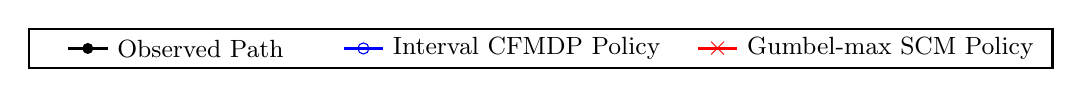
\begin{tikzpicture}[scale=1.0, every node/.style={scale=1.0}]
            \draw[thick, black] (-3, -0.25) rectangle (10, 0.25);
            %
            \draw[black, line width=1pt] (-2.5, 0.0) -- (-2,0.0);
            \fill[black] (-2.25,0.0) circle (2pt); %
            \node[right] at (-2,0.0) {\small Observed Path};
            
            %
            \draw[blue, line width=1pt] (1.0,0.0) -- (1.5,0.0);
            \node[draw=blue, circle, minimum size=4pt, inner sep=0pt] at (1.25,0.0) {}; %
            \node[right] at (1.5,0.0) {\small Interval CFMDP Policy};
            
            %
            \draw[red, line width=1pt] (5.5,0) -- (6,0);
            \node[red] at (5.75,0) {$\boldsymbol{\times}$}; %
            \node[right] at (6,0) {\small Gumbel-max SCM Policy};
        \end{tikzpicture}
    }\\
    %
    \subfigure[\footnotesize Lowest cumulative reward: Interval CFMDP ($312$), Gumbel-max SCM ($312$)]{%
        \resizebox{0.76\columnwidth}{!}{
             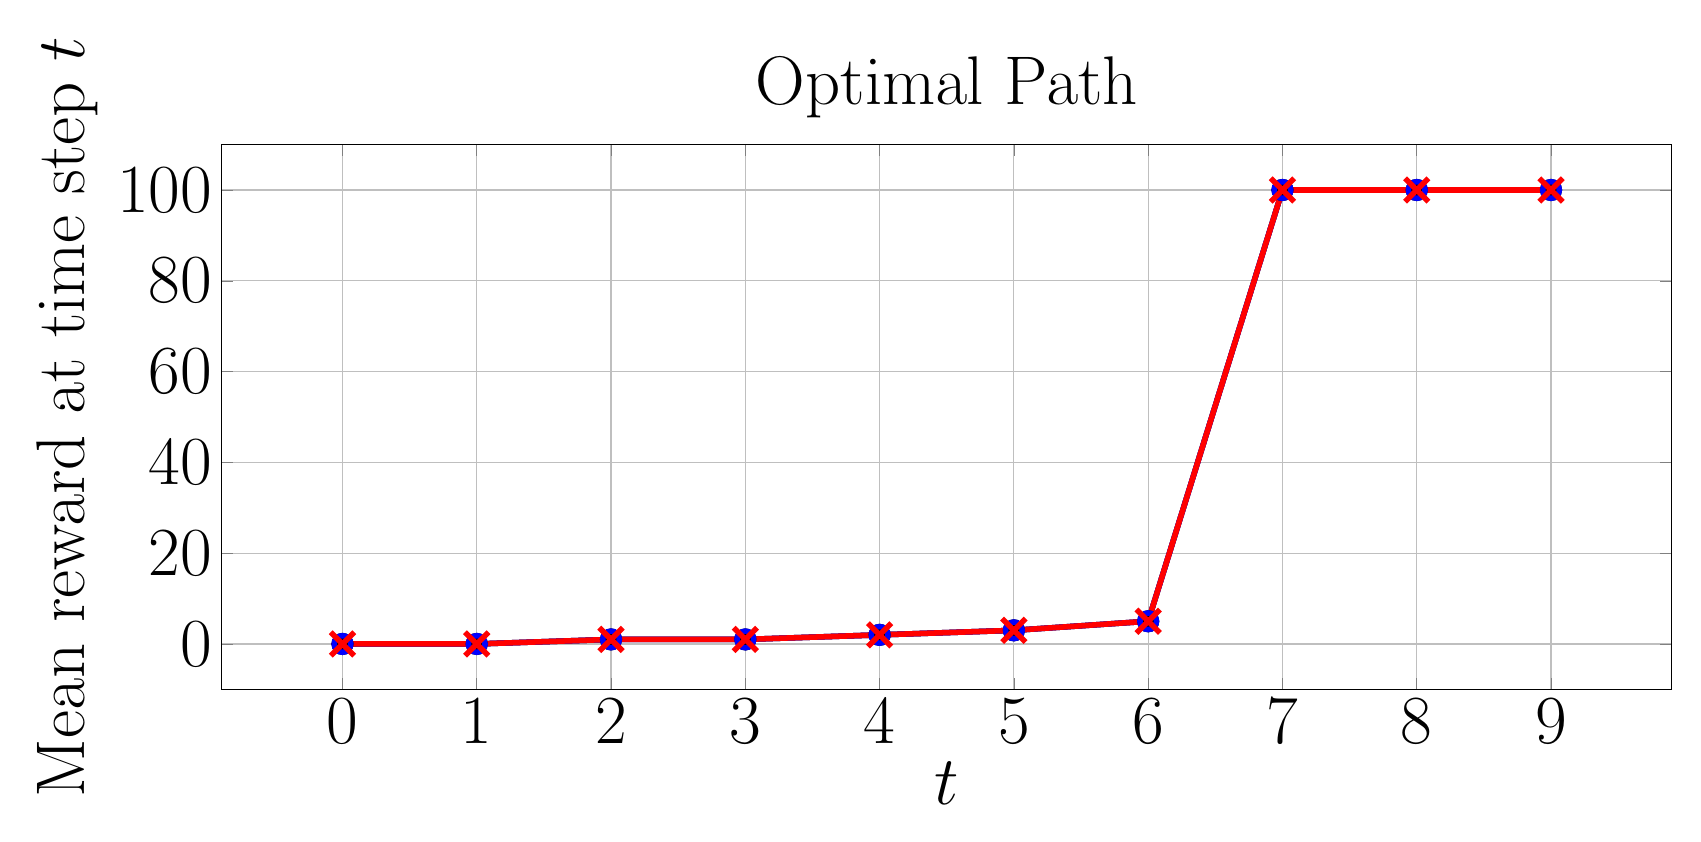
\begin{tikzpicture}
                \begin{axis}[
                    xlabel={$t$},
                    ylabel={Mean reward at time step $t$},
                    title={Optimal Path},
                    grid=both,
                    width=20cm, height=8.5cm,
                    every axis/.style={font=\Huge},
                    %
                ]
                \addplot[
                    color=black, %
                    mark=*, %
                    line width=2pt,
                    mark size=3pt,
                    error bars/.cd,
                    y dir=both, %
                    y explicit, %
                    error bar style={line width=1pt,solid},
                    error mark options={line width=1pt,mark size=4pt,rotate=90}
                ]
                coordinates {
                    (0, 0.0)  +- (0, 0.0)
                    (1, 0.0)  +- (0, 0.0) 
                    (2, 1.0)  +- (0, 0.0) 
                    (3, 1.0)  +- (0, 0.0)
                    (4, 2.0)  +- (0, 0.0)
                    (5, 3.0) +- (0, 0.0)
                    (6, 5.0) +- (0, 0.0)
                    (7, 100.0) +- (0, 0.0)
                    (8, 100.0) +- (0, 0.0)
                    (9, 100.0) +- (0, 0.0)
                };
                %
                \addplot[
                    color=blue, %
                    mark=o, %
                    line width=2pt,
                    mark size=3pt,
                    error bars/.cd,
                    y dir=both, %
                    y explicit, %
                    error bar style={line width=1pt,solid},
                    error mark options={line width=1pt,mark size=4pt,rotate=90}
                ]
                 coordinates {
                    (0, 0.0)  +- (0, 0.0)
                    (1, 0.0)  +- (0, 0.0) 
                    (2, 1.0)  +- (0, 0.0) 
                    (3, 1.0)  +- (0, 0.0)
                    (4, 2.0)  +- (0, 0.0)
                    (5, 3.0) +- (0, 0.0)
                    (6, 5.0) +- (0, 0.0)
                    (7, 100.0) +- (0, 0.0)
                    (8, 100.0) +- (0, 0.0)
                    (9, 100.0) +- (0, 0.0)
                };
                %
                \addplot[
                    color=red, %
                    mark=x, %
                    line width=2pt,
                    mark size=6pt,
                    error bars/.cd,
                    y dir=both, %
                    y explicit, %
                    error bar style={line width=1pt,solid},
                    error mark options={line width=1pt,mark size=4pt,rotate=90}
                ]
                coordinates {
                    (0, 0.0)  +- (0, 0.0)
                    (1, 0.0)  +- (0, 0.0) 
                    (2, 1.0)  +- (0, 0.0) 
                    (3, 1.0)  +- (0, 0.0)
                    (4, 2.0)  +- (0, 0.0)
                    (5, 3.0) +- (0, 0.0)
                    (6, 5.0) +- (0, 0.0)
                    (7, 100.0) +- (0, 0.0)
                    (8, 100.0) +- (0, 0.0)
                    (9, 100.0) +- (0, 0.0)
                };
                \end{axis}
            \end{tikzpicture}
         }
    }
    \hspace{1cm}
    \subfigure[\footnotesize Lowest cumulative reward: Interval CFMDP ($19$), Gumbel-max SCM ($-88$)]{%
         \resizebox{0.76\columnwidth}{!}{
            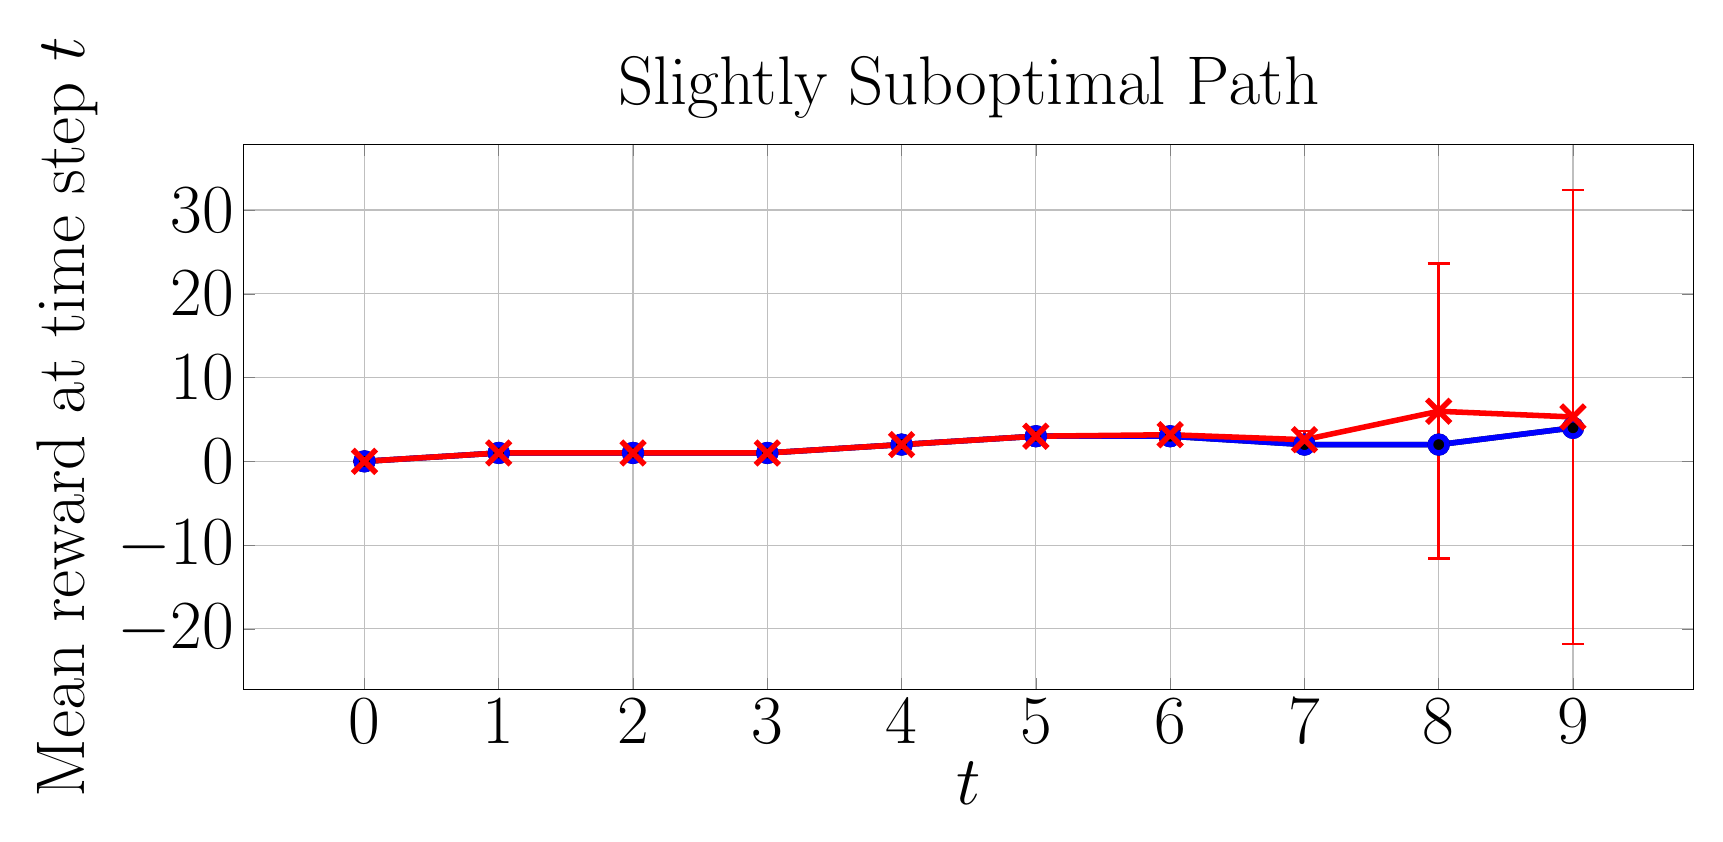
\begin{tikzpicture}
                \begin{axis}[
                    xlabel={$t$},
                    ylabel={Mean reward at time step $t$},
                    title={Slightly Suboptimal Path},
                    grid=both,
                    width=20cm, height=8.5cm,
                    every axis/.style={font=\Huge},
                    %
                ]
                \addplot[
                    color=black, %
                    mark=*, %
                    line width=2pt,
                    mark size=3pt,
                    error bars/.cd,
                    y dir=both, %
                    y explicit, %
                    error bar style={line width=1pt,solid},
                    error mark options={line width=1pt,mark size=4pt,rotate=90}
                ]
              coordinates {
                    (0, 0.0)  +- (0, 0.0)
                    (1, 1.0)  +- (0, 0.0) 
                    (2, 1.0)  +- (0, 0.0) 
                    (3, 1.0)  +- (0, 0.0)
                    (4, 2.0)  +- (0, 0.0)
                    (5, 3.0) +- (0, 0.0)
                    (6, 3.0) +- (0, 0.0)
                    (7, 2.0) +- (0, 0.0)
                    (8, 2.0) +- (0, 0.0)
                    (9, 4.0) +- (0, 0.0)
                };
                %
                \addplot[
                    color=blue, %
                    mark=o, %
                    line width=2pt,
                    mark size=3pt,
                    error bars/.cd,
                    y dir=both, %
                    y explicit, %
                    error bar style={line width=1pt,solid},
                    error mark options={line width=1pt,mark size=4pt,rotate=90}
                ]
              coordinates {
                    (0, 0.0)  +- (0, 0.0)
                    (1, 1.0)  +- (0, 0.0) 
                    (2, 1.0)  +- (0, 0.0) 
                    (3, 1.0)  +- (0, 0.0)
                    (4, 2.0)  +- (0, 0.0)
                    (5, 3.0) +- (0, 0.0)
                    (6, 3.0) +- (0, 0.0)
                    (7, 2.0) +- (0, 0.0)
                    (8, 2.0) +- (0, 0.0)
                    (9, 4.0) +- (0, 0.0)
                };
                %
                \addplot[
                    color=red, %
                    mark=x, %
                    line width=2pt,
                    mark size=6pt,
                    error bars/.cd,
                    y dir=both, %
                    y explicit, %
                    error bar style={line width=1pt,solid},
                    error mark options={line width=1pt,mark size=4pt,rotate=90}
                ]
                coordinates {
                    (0, 0.0)  +- (0, 0.0)
                    (1, 1.0)  +- (0, 0.0) 
                    (2, 1.0)  +- (0, 0.0) 
                    (3, 1.0)  +- (0, 0.0)
                    (4, 2.0)  += (0, 0.0)
                    (5, 3.0)  += (0, 0.0)
                    (6, 3.17847) += (0, 0.62606746) -= (0, 0.62606746)
                    (7, 2.5832885) += (0, 1.04598233) -= (0, 1.04598233)
                    (8, 5.978909) += (0, 17.60137623) -= (0, 17.60137623)
                    (9, 5.297059) += (0, 27.09227512) -= (0, 27.09227512)
                };
                \end{axis}
            \end{tikzpicture}
         }
    }\\[-1.5pt]
    \subfigure[\footnotesize Lowest cumulative reward: Interval CFMDP ($14$), Gumbel-max SCM ($-598$)]{%
         \resizebox{0.76\columnwidth}{!}{
             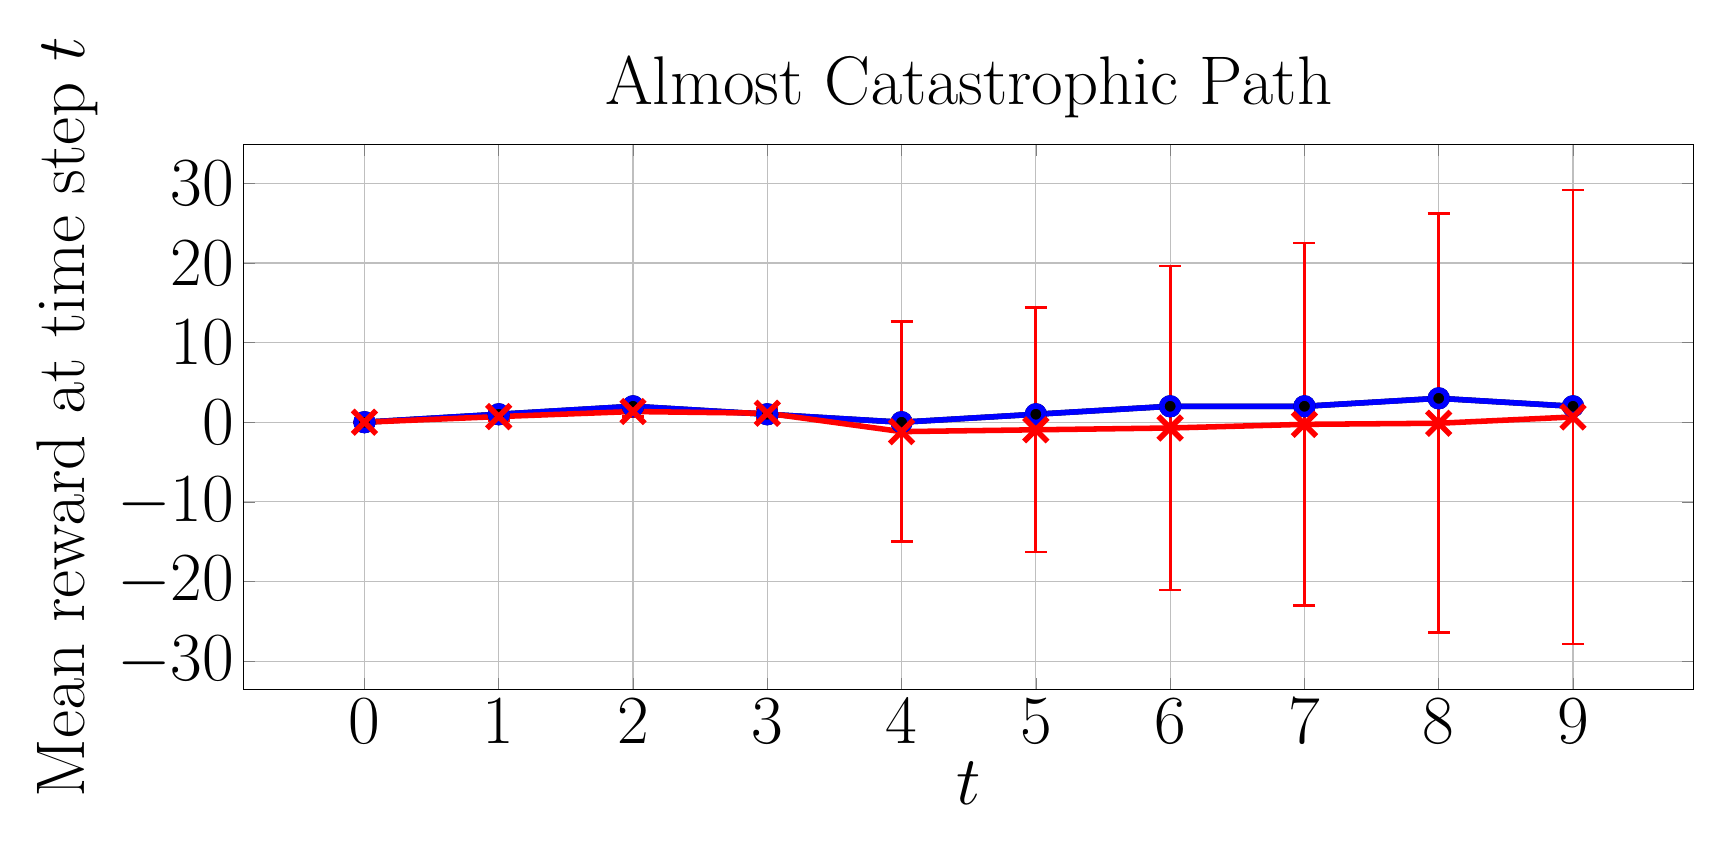
\begin{tikzpicture}
                \begin{axis}[
                    xlabel={$t$},
                    ylabel={Mean reward at time step $t$},
                    title={Almost Catastrophic Path},
                    grid=both,
                    width=20cm, height=8.5cm,
                    every axis/.style={font=\Huge},
                    %
                ]
                \addplot[
                    color=black, %
                    mark=*, %
                    line width=2pt,
                    mark size=3pt,
                    error bars/.cd,
                    y dir=both, %
                    y explicit, %
                    error bar style={line width=1pt,solid},
                    error mark options={line width=1pt,mark size=4pt,rotate=90}
                ]
                coordinates {
                    (0, 0.0)  +- (0, 0.0)
                    (1, 1.0)  +- (0, 0.0) 
                    (2, 2.0)  +- (0, 0.0) 
                    (3, 1.0)  +- (0, 0.0)
                    (4, 0.0)  +- (0, 0.0)
                    (5, 1.0) +- (0, 0.0)
                    (6, 2.0) +- (0, 0.0)
                    (7, 2.0) +- (0, 0.0)
                    (8, 3.0) +- (0, 0.0)
                    (9, 2.0) +- (0, 0.0)
                };
                %
                \addplot[
                    color=blue, %
                    mark=o, %
                    line width=2pt,
                    mark size=3pt,
                    error bars/.cd,
                    y dir=both, %
                    y explicit, %
                    error bar style={line width=1pt,solid},
                    error mark options={line width=1pt,mark size=4pt,rotate=90}
                ]
                coordinates {
                    (0, 0.0)  +- (0, 0.0)
                    (1, 1.0)  +- (0, 0.0) 
                    (2, 2.0)  +- (0, 0.0) 
                    (3, 1.0)  +- (0, 0.0)
                    (4, 0.0)  +- (0, 0.0)
                    (5, 1.0) +- (0, 0.0)
                    (6, 2.0) +- (0, 0.0)
                    (7, 2.0) +- (0, 0.0)
                    (8, 3.0) +- (0, 0.0)
                    (9, 2.0) +- (0, 0.0)
                };
                %
                \addplot[
                    color=red, %
                    mark=x, %
                    line width=2pt,
                    mark size=6pt,
                    error bars/.cd,
                    y dir=both, %
                    y explicit, %
                    error bar style={line width=1pt,solid},
                    error mark options={line width=1pt,mark size=4pt,rotate=90}
                ]
                coordinates {
                    (0, 0.0)  +- (0, 0.0)
                    (1, 0.7065655)  +- (0, 0.4553358) 
                    (2, 1.341673)  +- (0, 0.67091621) 
                    (3, 1.122926)  +- (0, 0.61281824)
                    (4, -1.1821935)  +- (0, 13.82444042)
                    (5, -0.952399)  +- (0, 15.35195457)
                    (6, -0.72672) +- (0, 20.33508414)
                    (7, -0.268983) +- (0, 22.77861454)
                    (8, -0.1310835) +- (0, 26.31013314)
                    (9, 0.65806) +- (0, 28.50670214)
                };
                %
            %
            %
            %
            %
            %
            %
            %
            %
            %
            %
            %
            %
            %
            %
            %
            %
            %
            %
                \end{axis}
            \end{tikzpicture}
         }
    }
    \hspace{1cm}
    \subfigure[\footnotesize Lowest cumulative reward: Interval CFMDP ($-698$), Gumbel-max SCM ($-698$)]{%
         \resizebox{0.76\columnwidth}{!}{
            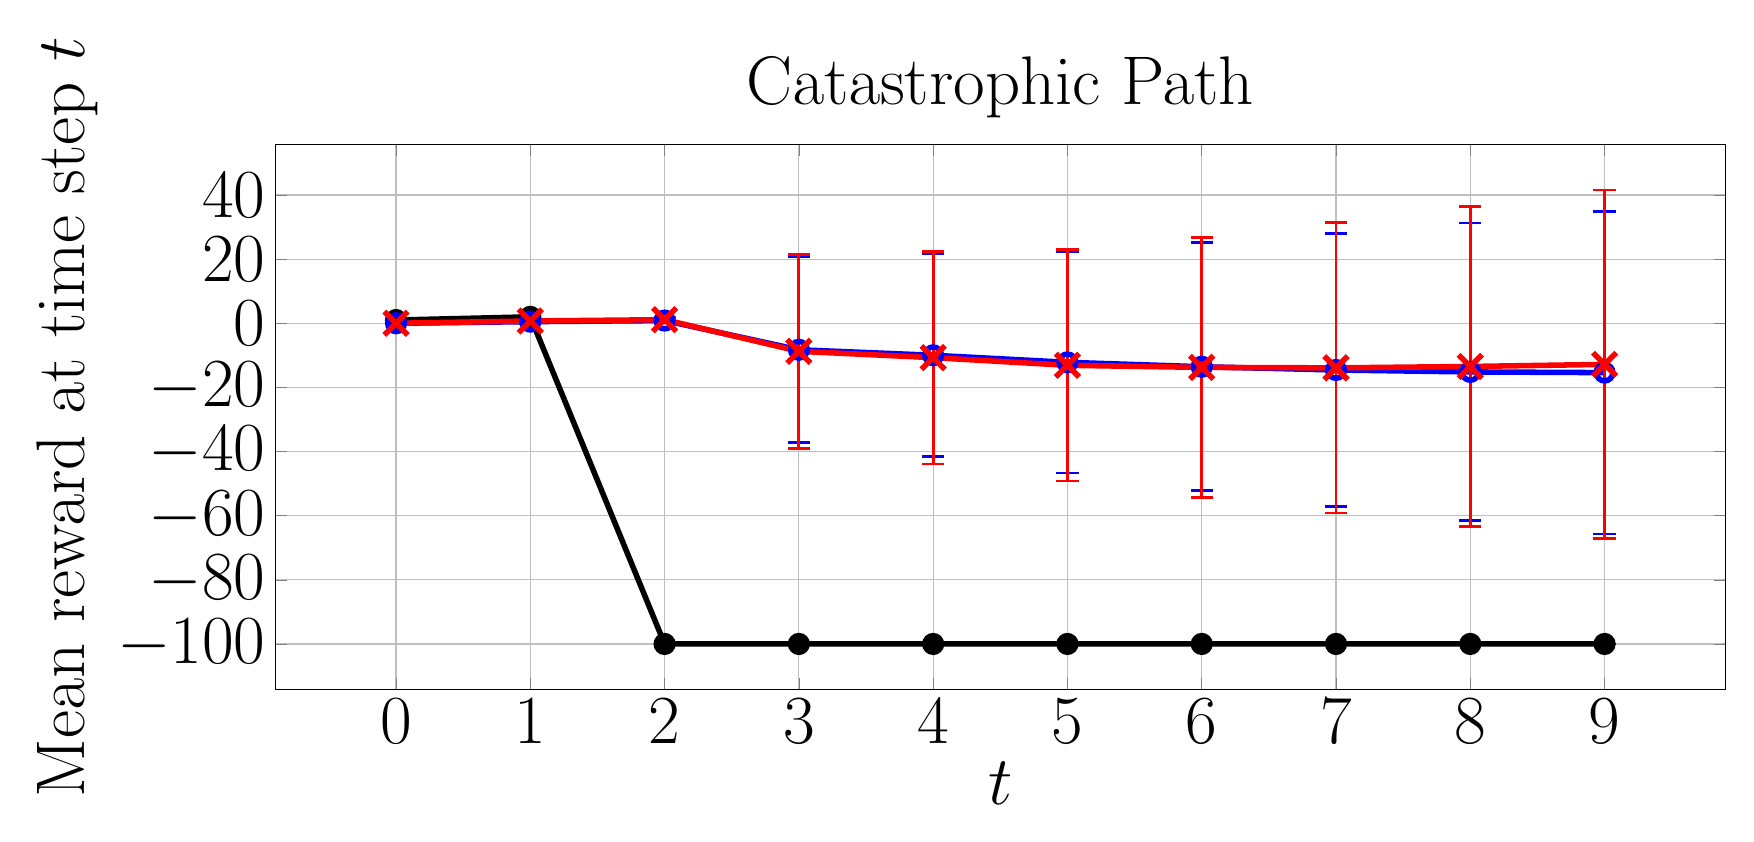
\begin{tikzpicture}
                \begin{axis}[
                    xlabel={$t$},
                    ylabel={Mean reward at time step $t$},
                    title={Catastrophic Path},
                    grid=both,
                    width=20cm, height=8.5cm,
                    every axis/.style={font=\Huge},
                    %
                ]
                \addplot[
                    color=black, %
                    mark=*, %
                    line width=2pt,
                    mark size=3pt,
                    error bars/.cd,
                    y dir=both, %
                    y explicit, %
                    error bar style={line width=1pt,solid},
                    error mark options={line width=1pt,mark size=4pt,rotate=90}
                ]
                coordinates {
                    (0, 1.0)  +- (0, 0.0)
                    (1, 2.0)  +- (0, 0.0) 
                    (2, -100.0)  +- (0, 0.0) 
                    (3, -100.0)  +- (0, 0.0)
                    (4, -100.0)  +- (0, 0.0)
                    (5, -100.0) +- (0, 0.0)
                    (6, -100.0) +- (0, 0.0)
                    (7, -100.0) +- (0, 0.0)
                    (8, -100.0) +- (0, 0.0)
                    (9, -100.0) +- (0, 0.0)
                };
                %
                \addplot[
                    color=blue, %
                    mark=o, %
                    line width=2pt,
                    mark size=3pt,
                    error bars/.cd,
                    y dir=both, %
                    y explicit, %
                    error bar style={line width=1pt,solid},
                    error mark options={line width=1pt,mark size=4pt,rotate=90}
                ]
                coordinates {
                    (0, 0.0)  +- (0, 0.0)
                    (1, 0.504814)  +- (0, 0.49997682) 
                    (2, 0.8439835)  +- (0, 0.76831917) 
                    (3, -8.2709165)  +- (0, 28.93656754)
                    (4, -9.981082)  +- (0, 31.66825363)
                    (5, -12.1776325) +- (0, 34.53463233)
                    (6, -13.556076) +- (0, 38.62845372)
                    (7, -14.574418) +- (0, 42.49603359)
                    (8, -15.1757075) +- (0, 46.41913968)
                    (9, -15.3900395) +- (0, 50.33563368)
                };
                %
                \addplot[
                    color=red, %
                    mark=x, %
                    line width=2pt,
                    mark size=6pt,
                    error bars/.cd,
                    y dir=both, %
                    y explicit, %
                    error bar style={line width=1pt,solid},
                    error mark options={line width=1pt,mark size=4pt,rotate=90}
                ]
                coordinates {
                    (0, 0.0)  +- (0, 0.0)
                    (1, 0.701873)  +- (0, 0.45743556) 
                    (2, 1.1227805)  +- (0, 0.73433129) 
                    (3, -8.7503255)  +- (0, 30.30257976)
                    (4, -10.722092)  +- (0, 33.17618589)
                    (5, -13.10721)  +- (0, 36.0648089)
                    (6, -13.7631645) +- (0, 40.56553451)
                    (7, -13.909043) +- (0, 45.23829402)
                    (8, -13.472517) +- (0, 49.96270296)
                    (9, -12.8278835) +- (0, 54.38618735)
                };
                %
            %
            %
            %
            %
            %
            %
            %
            %
            %
            %
            %
            %
            %
            %
            %
            %
            %
            %
                \end{axis}
            \end{tikzpicture}
         }
    }
    \caption{Average instant reward of CF paths induced by policies on GridWorld $p=0.4$.}
    \label{fig: reward p=0.4}
\end{figure*}

\subsection{Experimental Setup}
To compare policy performance, we measure the average rewards of counterfactual paths induced by our policy and the Gumbel-max policy by uniformly sampling $200$ counterfactual MDPs from the ICFMDP and generating $10,000$ counterfactual paths over each sampled CFMDP. \jl{Since the interval CFMDP depends on the observed path, we select $4$  paths of varying optimality to evaluate how the observed path impacts the performance of both policies: an optimal path, a slightly suboptimal path that could reach the optimal reward with a few changes, a catastrophic path that enters a catastrophic, terminal state with low reward, and an almost catastrophic path that was close to entering a catastrophic state.} When measuring the average probability bound widths and execution time needed to generate the ICFMDPs, we averaged over $20$ randomly generated observed paths
\footnote{Further training details are provided in Appendix \ref{app: training details}, and the code is provided at \href{https://github.com/ddv-lab/robust-cf-inference-in-MDPs}{https://github.com/ddv-lab/robust-cf-inference-in-MDPs}
%
%
.}.

\subsection{GridWorld}
\jl{The GridWorld MDP is a $4 \times 4$ grid where an agent must navigate from the top-left corner to the goal state in the bottom-right corner, avoiding a dangerous terminal state in the centre. At each time step, the agent can move up, down, left, or right, but there is a small probability (controlled by hyper-parameter $p$) of moving in an unintended direction. As the agent nears the goal, the reward for each state increases, culminating in a reward of $+100$ for reaching the goal. Entering the dangerous state results in a penalty of $-100$. We use two versions of GridWorld: a less stochastic version with $p=0.9$ (i.e., $90$\% chance of moving in the chosen direction) and a more stochastic version with $p=0.4$.}

\paragraph{GridWorld ($p=0.9$)}
When $p=0.9$, the counterfactual probability bounds are typically narrow (see Table \ref{tab:nonzero_probs} for average measurements). Consequently, as shown in Figure \ref{fig: reward p=0.9}, both policies are nearly identical and perform similarly well across the optimal, slightly suboptimal, and catastrophic paths.
%
However, for the almost catastrophic path, the interval CFMDP path is more conservative and follows the observed path more closely (as this is where the probability bounds are narrowest), which typically requires one additional step to reach the goal state than the Gumbel-max SCM policy.
%

\paragraph{GridWorld ($p=0.4$)}
\jl{When $p=0.4$, the GridWorld environment becomes more uncertain, increasing the risk of entering the dangerous state even if correct actions are chosen. Thus, as shown in Figure \ref{fig: reward p=0.4}, the interval CFMDP policy adopts a more conservative approach, avoiding deviation from the observed policy if it cannot guarantee higher counterfactual rewards (see the slightly suboptimal and almost catastrophic paths), whereas the Gumbel-max SCM is inconsistent: it can yield higher rewards, but also much lower rewards, reflected in the wide error bars.} For the catastrophic path, both policies must deviate from the observed path to achieve a higher reward and, in this case, perform similarly.
%
%
%
%
\subsection{Sepsis}
The Sepsis MDP \citep{oberst2019counterfactual} simulates trajectories of Sepsis patients. Each state consists of four vital signs (heart rate, blood pressure, oxygen concentration, and glucose levels), categorised as low, normal, or high.
and three treatments that can be toggled on/off at each time step (8 actions in total). Unlike \citet{oberst2019counterfactual}, we scale rewards based on the number of out-of-range vital signs, between $-1000$ (patient dies) and $1000$ (patient discharged). \jl{Like the GridWorld $p=0.4$ experiment, the Sepsis MDP is highly uncertain, as many states are equally likely to lead to optimal and poor outcomes. Thus, as shown in Figure \ref{fig: reward sepsis}, both policies follow the observed optimal and almost catastrophic paths to guarantee rewards are no worse than the observation.} However, improving the catastrophic path requires deviating from the observation. Here, the Gumbel-max SCM policy, on average, performs better than the interval CFMDP policy. But, since both policies have lower bounds clipped at $-1000$, neither policy reliably improves over the observation. In contrast, for the slightly suboptimal path, the interval CFMDP policy performs significantly better, shown by its higher lower bounds. 
Moreover, in these two cases, the worst-case counterfactual path generated by the interval CFMDP policy is better than that of the Gumbel-max SCM policy,
indicating its greater robustness.
%
\begin{figure*}
    \centering
     \resizebox{0.6\textwidth}{!}{
        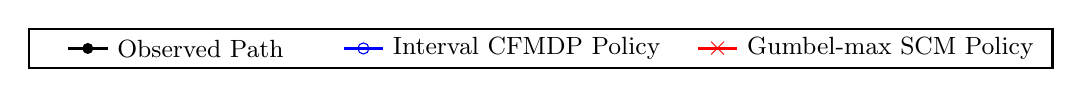
\begin{tikzpicture}[scale=1.0, every node/.style={scale=1.0}]
            \draw[thick, black] (-3, -0.25) rectangle (10, 0.25);
            %
            \draw[black, line width=1pt] (-2.5, 0.0) -- (-2,0.0);
            \fill[black] (-2.25,0.0) circle (2pt); %
            \node[right] at (-2,0.0) {\small Observed Path};
            
            %
            \draw[blue, line width=1pt] (1.0,0.0) -- (1.5,0.0);
            \node[draw=blue, circle, minimum size=4pt, inner sep=0pt] at (1.25,0.0) {}; %
            \node[right] at (1.5,0.0) {\small Interval CFMDP Policy};
            
            %
            \draw[red, line width=1pt] (5.5,0) -- (6,0);
            \node[red] at (5.75,0) {$\boldsymbol{\times}$}; %
            \node[right] at (6,0) {\small Gumbel-max SCM Policy};
        \end{tikzpicture}
    }\\
    \subfigure[\footnotesize Lowest cumulative reward: Interval CFMDP ($8000$), Gumbel-max SCM ($8000$)]{%
         \resizebox{0.76\columnwidth}{!}{
             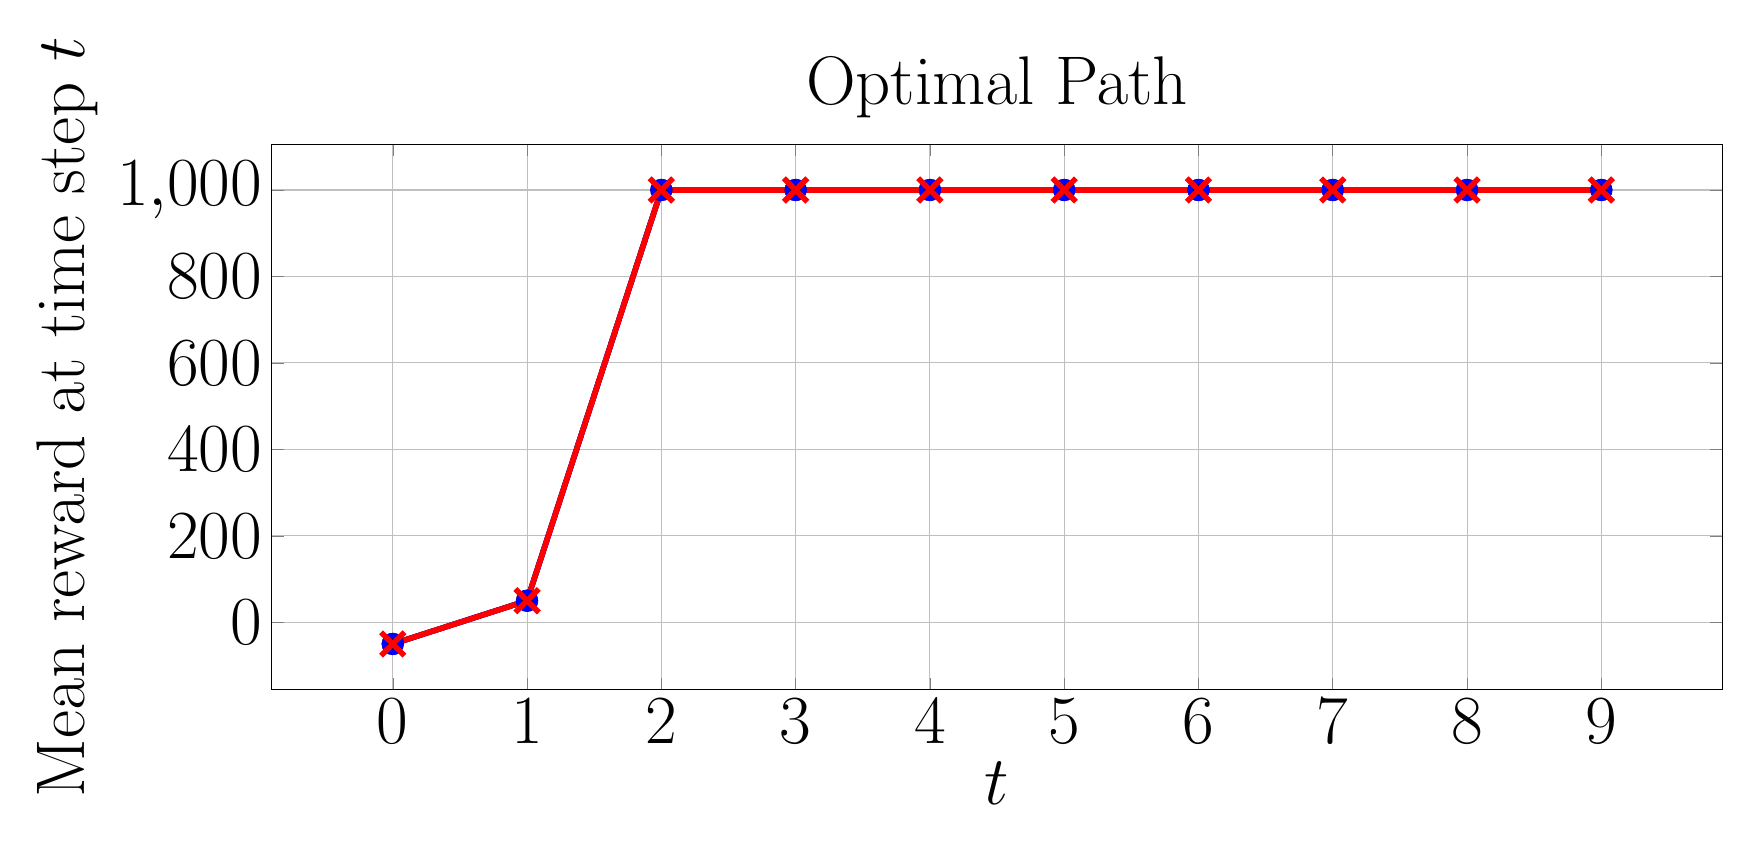
\begin{tikzpicture}
                \begin{axis}[
                    xlabel={$t$},
                    ylabel={Mean reward at time step $t$},
                    title={Optimal Path},
                    grid=both,
                    width=20cm, height=8.5cm,
                    every axis/.style={font=\Huge},
                    %
                ]
                \addplot[
                    color=black, %
                    mark=*, %
                    line width=2pt,
                    mark size=3pt,
                ]
                coordinates {
                    (0, -50.0)
                    (1, 50.0)
                    (2, 1000.0)
                    (3, 1000.0)
                    (4, 1000.0)
                    (5, 1000.0)
                    (6, 1000.0)
                    (7, 1000.0)
                    (8, 1000.0)
                    (9, 1000.0)
                };
                %
                \addplot[
                    color=blue, %
                    mark=o, %
                    line width=2pt,
                    mark size=3pt,
                    error bars/.cd,
                    y dir=both, %
                    y explicit, %
                    error bar style={line width=1pt,solid},
                    error mark options={line width=1pt,mark size=4pt,rotate=90}
                ]
                coordinates {
                    (0, -50.0)  +- (0, 0.0)
                    (1, 50.0)  +- (0, 0.0) 
                    (2, 1000.0)  +- (0, 0.0) 
                    (3, 1000.0)  +- (0, 0.0)
                    (4, 1000.0)  +- (0, 0.0)
                    (5, 1000.0) +- (0, 0.0)
                    (6, 1000.0) +- (0, 0.0)
                    (7, 1000.0) +- (0, 0.0)
                    (8, 1000.0) +- (0, 0.0)
                    (9, 1000.0) +- (0, 0.0)
                };
                %
                \addplot[
                    color=red, %
                    mark=x, %
                    line width=2pt,
                    mark size=6pt,
                    error bars/.cd,
                    y dir=both, %
                    y explicit, %
                    error bar style={line width=1pt,solid},
                    error mark options={line width=1pt,mark size=4pt,rotate=90}
                ]
                coordinates {
                    (0, -50.0)  +- (0, 0.0)
                    (1, 50.0)  +- (0, 0.0) 
                    (2, 1000.0)  +- (0, 0.0) 
                    (3, 1000.0)  +- (0, 0.0)
                    (4, 1000.0)  +- (0, 0.0)
                    (5, 1000.0) +- (0, 0.0)
                    (6, 1000.0) +- (0, 0.0)
                    (7, 1000.0) +- (0, 0.0)
                    (8, 1000.0) +- (0, 0.0)
                    (9, 1000.0) +- (0, 0.0)
                };
                %
                \end{axis}
            \end{tikzpicture}
         }
    }
    \hspace{1cm}
    \subfigure[\footnotesize Lowest cumulative reward: Interval CFMDP ($-5980$), Gumbel-max SCM ($-8000$)]{%
         \resizebox{0.76\columnwidth}{!}{
            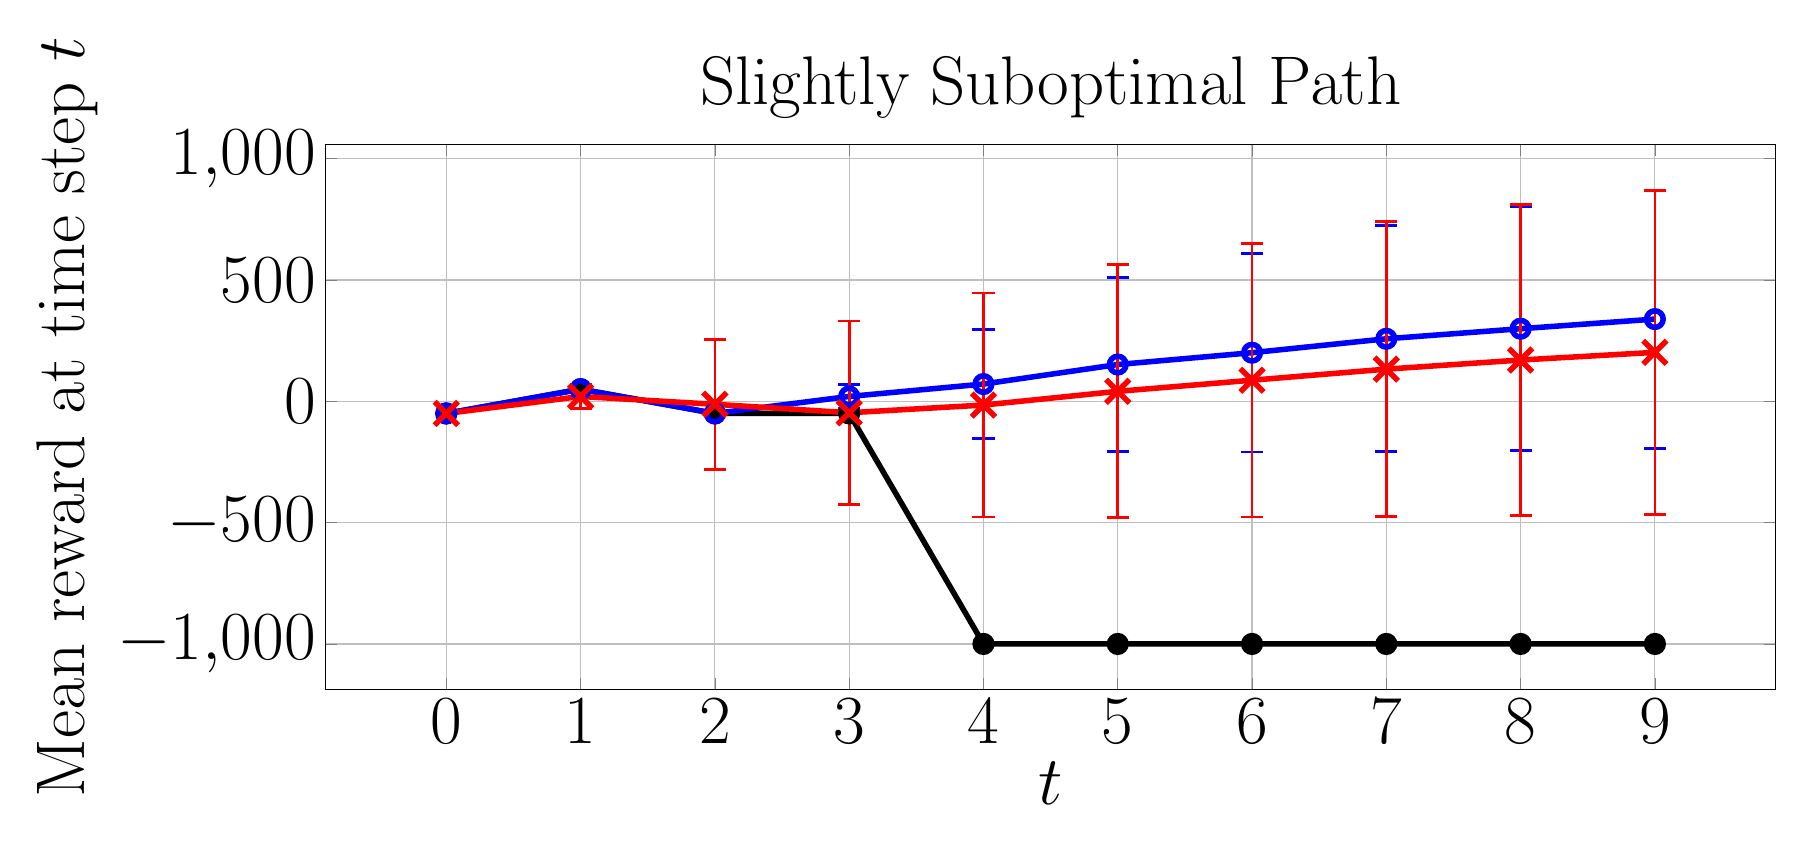
\begin{tikzpicture}
                \begin{axis}[
                    xlabel={$t$},
                    ylabel={Mean reward at time step $t$},
                    title={Slightly Suboptimal Path},
                    grid=both,
                    width=20cm, height=8.5cm,
                    every axis/.style={font=\Huge},
                    %
                ]
               \addplot[
                    color=black, %
                    mark=*, %
                    line width=2pt,
                    mark size=3pt,
                ]
                coordinates {
                    (0, -50.0)
                    (1, 50.0)
                    (2, -50.0)
                    (3, -50.0)
                    (4, -1000.0)
                    (5, -1000.0)
                    (6, -1000.0)
                    (7, -1000.0)
                    (8, -1000.0)
                    (9, -1000.0)
                };
                %
                \addplot[
                    color=blue, %
                    mark=o, %
                    line width=2pt,
                    mark size=3pt,
                    error bars/.cd,
                    y dir=both, %
                    y explicit, %
                    error bar style={line width=1pt,solid},
                    error mark options={line width=1pt,mark size=4pt,rotate=90}
                ]
                coordinates {
                    (0, -50.0)  +- (0, 0.0)
                    (1, 50.0)  +- (0, 0.0) 
                    (2, -50.0)  +- (0, 0.0) 
                    (3, 20.0631)  +- (0, 49.97539413)
                    (4, 71.206585)  +- (0, 226.02033693)
                    (5, 151.60797) +- (0, 359.23292559)
                    (6, 200.40593) +- (0, 408.86185176)
                    (7, 257.77948) +- (0, 466.10372804)
                    (8, 299.237465) +- (0, 501.82579506)
                    (9, 338.9129) +- (0, 532.06124996)
                };
                %
                \addplot[
                    color=red, %
                    mark=x, %
                    line width=2pt,
                    mark size=6pt,
                    error bars/.cd,
                    y dir=both, %
                    y explicit, %
                    error bar style={line width=1pt,solid},
                    error mark options={line width=1pt,mark size=4pt,rotate=90}
                ]
                coordinates {
                    (0, -50.0)  +- (0, 0.0)
                    (1, 20.00736)  +- (0, 49.99786741) 
                    (2, -12.282865)  +- (0, 267.598755) 
                    (3, -47.125995)  +- (0, 378.41755832)
                    (4, -15.381965)  +- (0, 461.77616558)
                    (5, 41.15459) +- (0, 521.53189262)
                    (6, 87.01595) +- (0, 564.22243126 )
                    (7, 132.62376) +- (0, 607.31338037)
                    (8, 170.168145) +- (0, 641.48013693)
                    (9, 201.813135) +- (0, 667.29441777)
                };
                %
                %
                %
                %
                %
                %
                %
                %
                %
                %
                %
                %
                %
                %
                %
                %
                %
                %
                %
                \end{axis}
            \end{tikzpicture}
         }
    }\\[-1.5pt]
    \subfigure[\footnotesize Lowest cumulative reward: Interval CFMDP ($100$), Gumbel-max SCM ($100$)]{%
         \resizebox{0.76\columnwidth}{!}{
             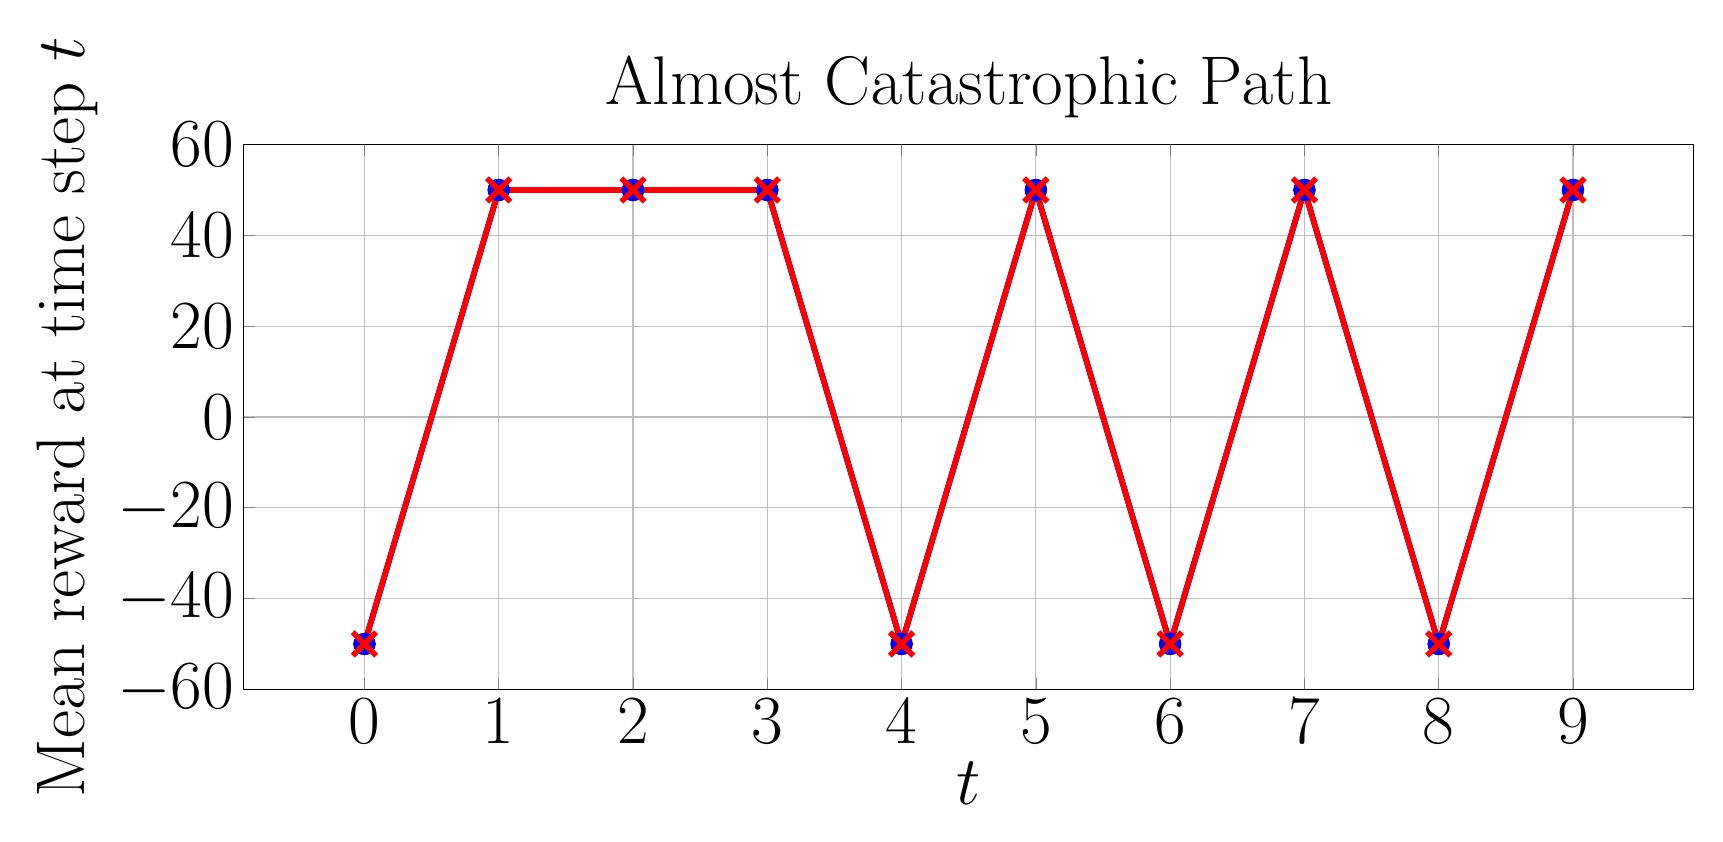
\begin{tikzpicture}
                \begin{axis}[
                    xlabel={$t$},
                    ylabel={Mean reward at time step $t$},
                    title={Almost Catastrophic Path},
                    grid=both,
                    every axis/.style={font=\Huge},
                    width=20cm, height=8.5cm,
                    %
                ]
               \addplot[
                    color=black, %
                    mark=*, %
                    line width=2pt,
                    mark size=3pt,
                ]
                coordinates {
                    (0, -50.0)
                    (1, 50.0)
                    (2, 50.0)
                    (3, 50.0)
                    (4, -50.0)
                    (5, 50.0)
                    (6, -50.0)
                    (7, 50.0)
                    (8, -50.0)
                    (9, 50.0)
                };
                %
                %
                \addplot[
                    color=blue, %
                    mark=o, %
                    line width=2pt,
                    mark size=3pt,
                    error bars/.cd,
                    y dir=both, %
                    y explicit, %
                    error bar style={line width=1pt,solid},
                    error mark options={line width=1pt,mark size=4pt,rotate=90}
                ]
                coordinates {
                    (0, -50.0)  +- (0, 0.0)
                    (1, 50.0)  +- (0, 0.0) 
                    (2, 50.0)  +- (0, 0.0) 
                    (3, 50.0)  +- (0, 0.0)
                    (4, -50.0)  +- (0, 0.0)
                    (5, 50.0) +- (0, 0.0)
                    (6, -50.0) +- (0, 0.0)
                    (7, 50.0) +- (0, 0.0)
                    (8, -50.0) +- (0, 0.0)
                    (9, 50.0) +- (0, 0.0)
                };
                %
                \addplot[
                    color=red, %
                    mark=x, %
                    line width=2pt,
                    mark size=6pt,
                    error bars/.cd,
                    y dir=both, %
                    y explicit, %
                    error bar style={line width=1pt,solid},
                    error mark options={line width=1pt,mark size=4pt,rotate=90}
                ]
                coordinates {
                    (0, -50.0)  +- (0, 0.0)
                    (1, 50.0)  +- (0, 0.0) 
                    (2, 50.0)  +- (0, 0.0) 
                    (3, 50.0)  +- (0, 0.0)
                    (4, -50.0)  +- (0, 0.0)
                    (5, 50.0) +- (0, 0.0)
                    (6, -50.0) +- (0, 0.0)
                    (7, 50.0) +- (0, 0.0)
                    (8, -50.0) +- (0, 0.0)
                    (9, 50.0) +- (0, 0.0)
                };
                %
                %
                %
                %
                %
                %
                %
                %
                %
                %
                %
                %
                %
                %
                %
                %
                %
                %
                %
                \end{axis}
            \end{tikzpicture}
         }
    }
    \hspace{1cm}
    \subfigure[\footnotesize Lowest cumulative reward: Interval CFMDP ($-7150$), Gumbel-max SCM ($-9050$)]{%
         \resizebox{0.76\columnwidth}{!}{
            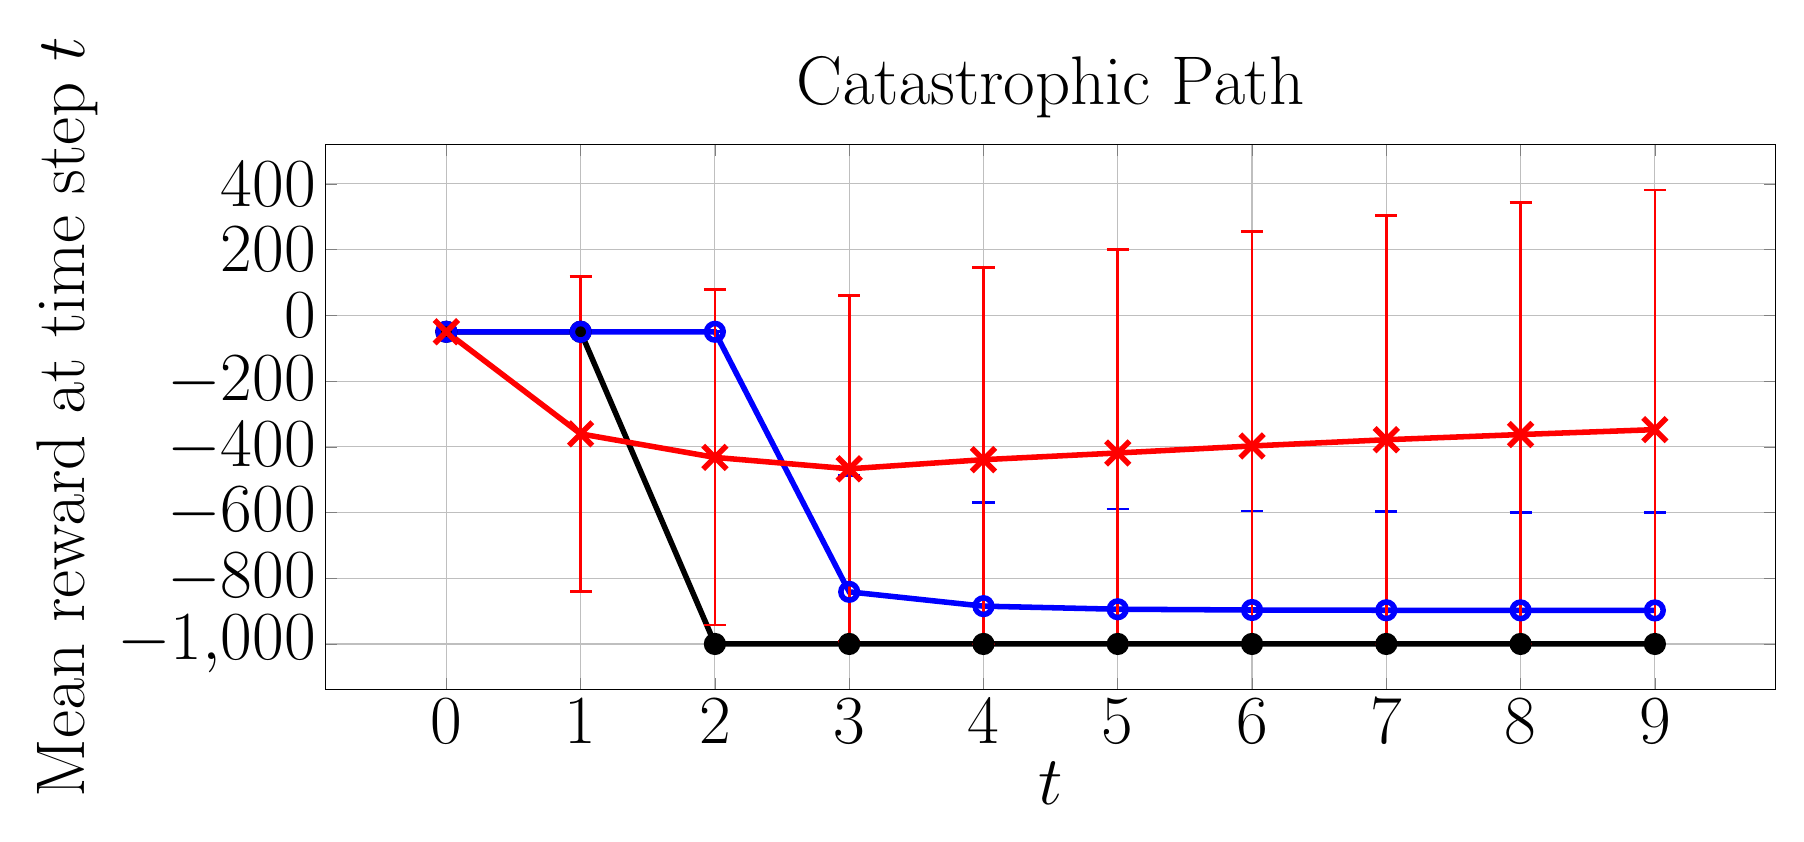
\begin{tikzpicture}
                \begin{axis}[
                    xlabel={$t$},
                    ylabel={Mean reward at time step $t$},
                    title={Catastrophic Path},
                    grid=both,
                    width=20cm, height=8.5cm,
                    every axis/.style={font=\Huge},
                    %
                ]
               \addplot[
                    color=black, %
                    mark=*, %
                    line width=2pt,
                    mark size=3pt,
                ]
                coordinates {
                    (0, -50.0)
                    (1, -50.0)
                    (2, -1000.0)
                    (3, -1000.0)
                    (4, -1000.0)
                    (5, -1000.0)
                    (6, -1000.0)
                    (7, -1000.0)
                    (8, -1000.0)
                    (9, -1000.0)
                };
                %
                %
                \addplot[
                    color=blue, %
                    mark=o, %
                    line width=2pt,
                    mark size=3pt,
                    error bars/.cd,
                    y dir=both, %
                    y explicit, %
                    error bar style={line width=1pt,solid},
                    error mark options={line width=1pt,mark size=4pt,rotate=90}
                ]
                coordinates {
                    (0, -50.0)  +- (0, 0.0)
                    (1, -50.0)  +- (0, 0.0) 
                    (2, -50.0)  +- (0, 0.0) 
                    (3, -841.440725)  += (0, 354.24605512) -= (0, 158.559275)
                    (4, -884.98225)  += (0, 315.37519669) -= (0, 115.01775)
                    (5, -894.330425) += (0, 304.88572805) -= (0, 105.669575)
                    (6, -896.696175) += (0, 301.19954514) -= (0, 103.303825)
                    (7, -897.4635) += (0, 299.61791279) -= (0, 102.5365)
                    (8, -897.77595) += (0, 298.80392585) -= (0, 102.22405)
                    (9, -897.942975) += (0, 298.32920557) -= (0, 102.057025)
                };
                %
                \addplot[
                    color=red, %
                    mark=x, %
                    line width=2pt,
                    mark size=6pt,
                    error bars/.cd,
                    y dir=both, %
                    y explicit, %
                    error bar style={line width=1pt,solid},
                    error mark options={line width=1pt,mark size=4pt,rotate=90}
                ]
            coordinates {
                    (0, -50.0)  +- (0, 0.0)
                    (1, -360.675265)  +- (0, 479.39812699) 
                    (2, -432.27629)  +- (0, 510.38620897) 
                    (3, -467.029545)  += (0, 526.36009628) -= (0, 526.36009628)
                    (4, -439.17429)  += (0, 583.96638919) -= (0, 560.82571)
                    (5, -418.82704) += (0, 618.43027478) -= (0, 581.17296)
                    (6, -397.464895) += (0, 652.67322574) -= (0, 602.535105)
                    (7, -378.49052) += (0, 682.85407033) -= (0, 621.50948)
                    (8, -362.654195) += (0, 707.01412023) -= (0, 637.345805)
                    (9, -347.737935) += (0, 729.29076479) -= (0, 652.262065)
                };
                %
                %
                %
                %
                %
                %
                %
                %
                %
                %
                %
                %
                %
                %
                %
                %
                %
                %
                %
                \end{axis}
            \end{tikzpicture}
         }
    }
    \caption{Average instant reward of CF paths induced by policies on Sepsis.}
    \label{fig: reward sepsis}
\end{figure*}

%
%
%
\subsection{Interval CFMDP Bounds}
%
%
Table \ref{tab:nonzero_probs} presents the mean counterfactual probability bound widths (excluding transitions where the upper bound is $0$) for each MDP, averaged over 20 observed paths. We compare the bounds under counterfactual stability (CS) and monotonicity (M) assumptions, CS alone, and no assumptions. This shows that the assumptions marginally reduce the bound widths, indicating the assumptions tighten the bounds without excluding too many causal models, as intended.
\renewcommand{\arraystretch}{1}

\begin{table}
\centering
\caption{Mean width of counterfactual probability bounds}
\resizebox{0.8\columnwidth}{!}{%
\begin{tabular}{|c|c|c|c|}
\hline
\multirow{2}{*}{\textbf{Environment}} & \multicolumn{3}{c|}{\textbf{Assumptions}} \\ \cline{2-4}
 & \textbf{CS + M} & \textbf{CS} & \textbf{None\tablefootnote{\jl{Equivalent to \citet{li2024probabilities}'s bounds (see Section \ref{sec: equivalence with Li}).}}} \\ \hline
\textbf{GridWorld} ($p=0.9$) & 0.0817 & 0.0977 & 0.100 \\ \hline
\textbf{GridWorld} ($p=0.4$) & 0.552  & 0.638  & 0.646 \\ \hline
\textbf{Sepsis} & 0.138 & 0.140 & 0.140 \\ \hline
\end{tabular}
}
\label{tab:nonzero_probs}
\end{table}


\subsection{Execution Times}
Table \ref{tab: times} compares the average time needed to generate the interval CFMDP vs.\ the Gumbel-max SCM CFMDP for 20 observations.
The GridWorld algorithms were run single-threaded, while the Sepsis experiments were run in parallel.
Generating the interval CFMDP is significantly faster as it uses exact analytical bounds, whereas the Gumbel-max CFMDP requires sampling from the Gumbel distribution to estimate counterfactual transition probabilities. \jl{Since constructing the counterfactual MDP models is the main bottleneck in both approaches, ours is more efficient overall and suitable for larger MDPs.}
\begin{table}
\centering
\caption{Mean execution time to generate CFMDPs}
\resizebox{0.99\columnwidth}{!}{%
\begin{tabular}{|c|c|c|}
\hline
\multirow{2}{*}{\textbf{Environment}} & \multicolumn{2}{c|}{\textbf{Mean Execution Time (s)}} \\ \cline{2-3} 
                                      & \textbf{Interval CFMDP} & \textbf{Gumbel-max CFMDP} \\ \hline
\textbf{GridWorld ($p=0.9$) }                  & 0.261                   & 56.1                      \\ \hline
\textbf{GridWorld ($p=0.4$)  }                 & 0.336                   & 54.5                      \\ \hline
\textbf{Sepsis}                                 & 688                     & 2940                      \\ \hline
\end{tabular}%
}
\label{tab: times}
\end{table}


\section{Related Work}
\label{sec:related_work}
\section{RELATED WORK}
\label{sec:relatedwork}
In this section, we describe the previous works related to our proposal, which are divided into two parts. In Section~\ref{sec:relatedwork_exoplanet}, we present a review of approaches based on machine learning techniques for the detection of planetary transit signals. Section~\ref{sec:relatedwork_attention} provides an account of the approaches based on attention mechanisms applied in Astronomy.\par

\subsection{Exoplanet detection}
\label{sec:relatedwork_exoplanet}
Machine learning methods have achieved great performance for the automatic selection of exoplanet transit signals. One of the earliest applications of machine learning is a model named Autovetter \citep{MCcauliff}, which is a random forest (RF) model based on characteristics derived from Kepler pipeline statistics to classify exoplanet and false positive signals. Then, other studies emerged that also used supervised learning. \cite{mislis2016sidra} also used a RF, but unlike the work by \citet{MCcauliff}, they used simulated light curves and a box least square \citep[BLS;][]{kovacs2002box}-based periodogram to search for transiting exoplanets. \citet{thompson2015machine} proposed a k-nearest neighbors model for Kepler data to determine if a given signal has similarity to known transits. Unsupervised learning techniques were also applied, such as self-organizing maps (SOM), proposed \citet{armstrong2016transit}; which implements an architecture to segment similar light curves. In the same way, \citet{armstrong2018automatic} developed a combination of supervised and unsupervised learning, including RF and SOM models. In general, these approaches require a previous phase of feature engineering for each light curve. \par

%DL is a modern data-driven technology that automatically extracts characteristics, and that has been successful in classification problems from a variety of application domains. The architecture relies on several layers of NNs of simple interconnected units and uses layers to build increasingly complex and useful features by means of linear and non-linear transformation. This family of models is capable of generating increasingly high-level representations \citep{lecun2015deep}.

The application of DL for exoplanetary signal detection has evolved rapidly in recent years and has become very popular in planetary science.  \citet{pearson2018} and \citet{zucker2018shallow} developed CNN-based algorithms that learn from synthetic data to search for exoplanets. Perhaps one of the most successful applications of the DL models in transit detection was that of \citet{Shallue_2018}; who, in collaboration with Google, proposed a CNN named AstroNet that recognizes exoplanet signals in real data from Kepler. AstroNet uses the training set of labelled TCEs from the Autovetter planet candidate catalog of Q1–Q17 data release 24 (DR24) of the Kepler mission \citep{catanzarite2015autovetter}. AstroNet analyses the data in two views: a ``global view'', and ``local view'' \citep{Shallue_2018}. \par


% The global view shows the characteristics of the light curve over an orbital period, and a local view shows the moment at occurring the transit in detail

%different = space-based

Based on AstroNet, researchers have modified the original AstroNet model to rank candidates from different surveys, specifically for Kepler and TESS missions. \citet{ansdell2018scientific} developed a CNN trained on Kepler data, and included for the first time the information on the centroids, showing that the model improves performance considerably. Then, \citet{osborn2020rapid} and \citet{yu2019identifying} also included the centroids information, but in addition, \citet{osborn2020rapid} included information of the stellar and transit parameters. Finally, \citet{rao2021nigraha} proposed a pipeline that includes a new ``half-phase'' view of the transit signal. This half-phase view represents a transit view with a different time and phase. The purpose of this view is to recover any possible secondary eclipse (the object hiding behind the disk of the primary star).


%last pipeline applies a procedure after the prediction of the model to obtain new candidates, this process is carried out through a series of steps that include the evaluation with Discovery and Validation of Exoplanets (DAVE) \citet{kostov2019discovery} that was adapted for the TESS telescope.\par
%



\subsection{Attention mechanisms in astronomy}
\label{sec:relatedwork_attention}
Despite the remarkable success of attention mechanisms in sequential data, few papers have exploited their advantages in astronomy. In particular, there are no models based on attention mechanisms for detecting planets. Below we present a summary of the main applications of this modeling approach to astronomy, based on two points of view; performance and interpretability of the model.\par
%Attention mechanisms have not yet been explored in all sub-areas of astronomy. However, recent works show a successful application of the mechanism.
%performance

The application of attention mechanisms has shown improvements in the performance of some regression and classification tasks compared to previous approaches. One of the first implementations of the attention mechanism was to find gravitational lenses proposed by \citet{thuruthipilly2021finding}. They designed 21 self-attention-based encoder models, where each model was trained separately with 18,000 simulated images, demonstrating that the model based on the Transformer has a better performance and uses fewer trainable parameters compared to CNN. A novel application was proposed by \citet{lin2021galaxy} for the morphological classification of galaxies, who used an architecture derived from the Transformer, named Vision Transformer (VIT) \citep{dosovitskiy2020image}. \citet{lin2021galaxy} demonstrated competitive results compared to CNNs. Another application with successful results was proposed by \citet{zerveas2021transformer}; which first proposed a transformer-based framework for learning unsupervised representations of multivariate time series. Their methodology takes advantage of unlabeled data to train an encoder and extract dense vector representations of time series. Subsequently, they evaluate the model for regression and classification tasks, demonstrating better performance than other state-of-the-art supervised methods, even with data sets with limited samples.

%interpretation
Regarding the interpretability of the model, a recent contribution that analyses the attention maps was presented by \citet{bowles20212}, which explored the use of group-equivariant self-attention for radio astronomy classification. Compared to other approaches, this model analysed the attention maps of the predictions and showed that the mechanism extracts the brightest spots and jets of the radio source more clearly. This indicates that attention maps for prediction interpretation could help experts see patterns that the human eye often misses. \par

In the field of variable stars, \citet{allam2021paying} employed the mechanism for classifying multivariate time series in variable stars. And additionally, \citet{allam2021paying} showed that the activation weights are accommodated according to the variation in brightness of the star, achieving a more interpretable model. And finally, related to the TESS telescope, \citet{morvan2022don} proposed a model that removes the noise from the light curves through the distribution of attention weights. \citet{morvan2022don} showed that the use of the attention mechanism is excellent for removing noise and outliers in time series datasets compared with other approaches. In addition, the use of attention maps allowed them to show the representations learned from the model. \par

Recent attention mechanism approaches in astronomy demonstrate comparable results with earlier approaches, such as CNNs. At the same time, they offer interpretability of their results, which allows a post-prediction analysis. \par



\section{Discussion \& Future Work}
\label{sec:discussion}
\section{Discussion of Assumptions}\label{sec:discussion}
In this paper, we have made several assumptions for the sake of clarity and simplicity. In this section, we discuss the rationale behind these assumptions, the extent to which these assumptions hold in practice, and the consequences for our protocol when these assumptions hold.

\subsection{Assumptions on the Demand}

There are two simplifying assumptions we make about the demand. First, we assume the demand at any time is relatively small compared to the channel capacities. Second, we take the demand to be constant over time. We elaborate upon both these points below.

\paragraph{Small demands} The assumption that demands are small relative to channel capacities is made precise in \eqref{eq:large_capacity_assumption}. This assumption simplifies two major aspects of our protocol. First, it largely removes congestion from consideration. In \eqref{eq:primal_problem}, there is no constraint ensuring that total flow in both directions stays below capacity--this is always met. Consequently, there is no Lagrange multiplier for congestion and no congestion pricing; only imbalance penalties apply. In contrast, protocols in \cite{sivaraman2020high, varma2021throughput, wang2024fence} include congestion fees due to explicit congestion constraints. Second, the bound \eqref{eq:large_capacity_assumption} ensures that as long as channels remain balanced, the network can always meet demand, no matter how the demand is routed. Since channels can rebalance when necessary, they never drop transactions. This allows prices and flows to adjust as per the equations in \eqref{eq:algorithm}, which makes it easier to prove the protocol's convergence guarantees. This also preserves the key property that a channel's price remains proportional to net money flow through it.

In practice, payment channel networks are used most often for micro-payments, for which on-chain transactions are prohibitively expensive; large transactions typically take place directly on the blockchain. For example, according to \cite{river2023lightning}, the average channel capacity is roughly $0.1$ BTC ($5,000$ BTC distributed over $50,000$ channels), while the average transaction amount is less than $0.0004$ BTC ($44.7k$ satoshis). Thus, the small demand assumption is not too unrealistic. Additionally, the occasional large transaction can be treated as a sequence of smaller transactions by breaking it into packets and executing each packet serially (as done by \cite{sivaraman2020high}).
Lastly, a good path discovery process that favors large capacity channels over small capacity ones can help ensure that the bound in \eqref{eq:large_capacity_assumption} holds.

\paragraph{Constant demands} 
In this work, we assume that any transacting pair of nodes have a steady transaction demand between them (see Section \ref{sec:transaction_requests}). Making this assumption is necessary to obtain the kind of guarantees that we have presented in this paper. Unless the demand is steady, it is unreasonable to expect that the flows converge to a steady value. Weaker assumptions on the demand lead to weaker guarantees. For example, with the more general setting of stochastic, but i.i.d. demand between any two nodes, \cite{varma2021throughput} shows that the channel queue lengths are bounded in expectation. If the demand can be arbitrary, then it is very hard to get any meaningful performance guarantees; \cite{wang2024fence} shows that even for a single bidirectional channel, the competitive ratio is infinite. Indeed, because a PCN is a decentralized system and decisions must be made based on local information alone, it is difficult for the network to find the optimal detailed balance flow at every time step with a time-varying demand.  With a steady demand, the network can discover the optimal flows in a reasonably short time, as our work shows.

We view the constant demand assumption as an approximation for a more general demand process that could be piece-wise constant, stochastic, or both (see simulations in Figure \ref{fig:five_nodes_variable_demand}).
We believe it should be possible to merge ideas from our work and \cite{varma2021throughput} to provide guarantees in a setting with random demands with arbitrary means. We leave this for future work. In addition, our work suggests that a reasonable method of handling stochastic demands is to queue the transaction requests \textit{at the source node} itself. This queuing action should be viewed in conjunction with flow-control. Indeed, a temporarily high unidirectional demand would raise prices for the sender, incentivizing the sender to stop sending the transactions. If the sender queues the transactions, they can send them later when prices drop. This form of queuing does not require any overhaul of the basic PCN infrastructure and is therefore simpler to implement than per-channel queues as suggested by \cite{sivaraman2020high} and \cite{varma2021throughput}.

\subsection{The Incentive of Channels}
The actions of the channels as prescribed by the DEBT control protocol can be summarized as follows. Channels adjust their prices in proportion to the net flow through them. They rebalance themselves whenever necessary and execute any transaction request that has been made of them. We discuss both these aspects below.

\paragraph{On Prices}
In this work, the exclusive role of channel prices is to ensure that the flows through each channel remains balanced. In practice, it would be important to include other components in a channel's price/fee as well: a congestion price  and an incentive price. The congestion price, as suggested by \cite{varma2021throughput}, would depend on the total flow of transactions through the channel, and would incentivize nodes to balance the load over different paths. The incentive price, which is commonly used in practice \cite{river2023lightning}, is necessary to provide channels with an incentive to serve as an intermediary for different channels. In practice, we expect both these components to be smaller than the imbalance price. Consequently, we expect the behavior of our protocol to be similar to our theoretical results even with these additional prices.

A key aspect of our protocol is that channel fees are allowed to be negative. Although the original Lightning network whitepaper \cite{poon2016bitcoin} suggests that negative channel prices may be a good solution to promote rebalancing, the idea of negative prices in not very popular in the literature. To our knowledge, the only prior work with this feature is \cite{varma2021throughput}. Indeed, in papers such as \cite{van2021merchant} and \cite{wang2024fence}, the price function is explicitly modified such that the channel price is never negative. The results of our paper show the benefits of negative prices. For one, in steady state, equal flows in both directions ensure that a channel doesn't loose any money (the other price components mentioned above ensure that the channel will only gain money). More importantly, negative prices are important to ensure that the protocol selectively stifles acyclic flows while allowing circulations to flow. Indeed, in the example of Section \ref{sec:flow_control_example}, the flows between nodes $A$ and $C$ are left on only because the large positive price over one channel is canceled by the corresponding negative price over the other channel, leading to a net zero price.

Lastly, observe that in the DEBT control protocol, the price charged by a channel does not depend on its capacity. This is a natural consequence of the price being the Lagrange multiplier for the net-zero flow constraint, which also does not depend on the channel capacity. In contrast, in many other works, the imbalance price is normalized by the channel capacity \cite{ren2018optimal, lin2020funds, wang2024fence}; this is shown to work well in practice. The rationale for such a price structure is explained well in \cite{wang2024fence}, where this fee is derived with the aim of always maintaining some balance (liquidity) at each end of every channel. This is a reasonable aim if a channel is to never rebalance itself; the experiments of the aforementioned papers are conducted in such a regime. In this work, however, we allow the channels to rebalance themselves a few times in order to settle on a detailed balance flow. This is because our focus is on the long-term steady state performance of the protocol. This difference in perspective also shows up in how the price depends on the channel imbalance. \cite{lin2020funds} and \cite{wang2024fence} advocate for strictly convex prices whereas this work and \cite{varma2021throughput} propose linear prices.

\paragraph{On Rebalancing} 
Recall that the DEBT control protocol ensures that the flows in the network converge to a detailed balance flow, which can be sustained perpetually without any rebalancing. However, during the transient phase (before convergence), channels may have to perform on-chain rebalancing a few times. Since rebalancing is an expensive operation, it is worthwhile discussing methods by which channels can reduce the extent of rebalancing. One option for the channels to reduce the extent of rebalancing is to increase their capacity; however, this comes at the cost of locking in more capital. Each channel can decide for itself the optimum amount of capital to lock in. Another option, which we discuss in Section \ref{sec:five_node}, is for channels to increase the rate $\gamma$ at which they adjust prices. 

Ultimately, whether or not it is beneficial for a channel to rebalance depends on the time-horizon under consideration. Our protocol is based on the assumption that the demand remains steady for a long period of time. If this is indeed the case, it would be worthwhile for a channel to rebalance itself as it can make up this cost through the incentive fees gained from the flow of transactions through it in steady state. If a channel chooses not to rebalance itself, however, there is a risk of being trapped in a deadlock, which is suboptimal for not only the nodes but also the channel.

\section{Conclusion}
This work presents DEBT control: a protocol for payment channel networks that uses source routing and flow control based on channel prices. The protocol is derived by posing a network utility maximization problem and analyzing its dual minimization. It is shown that under steady demands, the protocol guides the network to an optimal, sustainable point. Simulations show its robustness to demand variations. The work demonstrates that simple protocols with strong theoretical guarantees are possible for PCNs and we hope it inspires further theoretical research in this direction.

\section{Conclusion}
\label{sec:conclusion}
\section{Conclusion}
In this work, we propose a simple yet effective approach, called SMILE, for graph few-shot learning with fewer tasks. Specifically, we introduce a novel dual-level mixup strategy, including within-task and across-task mixup, for enriching the diversity of nodes within each task and the diversity of tasks. Also, we incorporate the degree-based prior information to learn expressive node embeddings. Theoretically, we prove that SMILE effectively enhances the model's generalization performance. Empirically, we conduct extensive experiments on multiple benchmarks and the results suggest that SMILE significantly outperforms other baselines, including both in-domain and cross-domain few-shot settings.

\bibliographystyle{ACM-Reference-Format}
\bibliography{refs}



\end{document}
\endinput
%%
%% End of file `sample-sigconf.tex'.
